\documentclass[12pt]{article}

\usepackage[margin=1in]{geometry}
\usepackage{amsmath, amssymb}
\usepackage{graphicx}
\usepackage{booktabs}
\usepackage{array}
\usepackage{caption}
\usepackage{subcaption}
\usepackage{hyperref}
\usepackage{natbib}
\usepackage{setspace}
\usepackage{float}
\usepackage[table]{xcolor}
\usepackage{microtype}
\usepackage{enumitem}

\hypersetup{
    colorlinks=true,
    linkcolor=blue!60!black,
    citecolor=blue!60!black,
    urlcolor=blue!60!black
}

\doublespacing

\title{\textbf{Selective Prediction and the Persistence Illusion:\\
A Diagnostic Decomposition of VIX Regime Classification}}

\author{
    Akshat Gupta \\
    \small Texas Academy of Mathematics and Science, University of North Texas \\
    \small Advisor: Dr.\ Jianguo Liu, Department of Mathematics, University of North Texas
}

\date{June 2026}

\begin{document}

\maketitle

\begin{abstract}
We present a three-part diagnostic protocol for evaluating selective prediction frameworks on autocorrelated classification labels: coverage-matched baseline comparison, regime-transition accuracy audit, and abstention confound testing. Applied to VIX regime classification over 5,000 trading days (2006--2026), the protocol shows that confidence-based selective prediction manufactures apparent skill by concentrating predictions on regime-stable days. Key findings: (1) the confidence filter achieves 0\% accuracy on every calm$\to$high volatility transition it covers, and explicit cost-weighting up to $20{\times}$ does not rescue this---the blindness is informational, not objective-function-driven; (2) at $N \geq 10$, Random Forest selective prediction and coverage-matched persistence make \emph{identical} predictions on every jointly covered day (McNemar $b = c = 0$), so the accuracy gap is attributable entirely to coverage composition, not multi-feature skill; (3) a HAR-style logistic regression on three VIX features matches or exceeds the 36-feature Random Forest in point estimate at four of five horizons, with no gap reaching statistical significance under moving-block bootstrap; (4) at $N = 25$, balanced accuracy collapses to 50\%, confirming that headline selective accuracy is an artifact of class imbalance, and (5) under any moderate false-negative cost asymmetry ($C \geq 5$), persistence at matched coverage dominates RF selective prediction on cost-weighted utility at $N = 10$. The protocol is modular and applicable to any selective prediction system on serially correlated labels.
\end{abstract}

\tableofcontents
\newpage

%-----------------------------------------------------------------------
\section{Introduction}
%-----------------------------------------------------------------------

Volatility is one of the most important dimensions of financial market risk. The CBOE Volatility Index (VIX), often described as the market's ``fear gauge,'' summarizes option-implied expectations of S\&P 500 volatility over the next 30 days and is widely used by investors, risk managers, and policymakers to monitor uncertainty in equity markets \citep{whaley2009}. When VIX rises above 20---a level widely adopted as a practical divide between normal and elevated-fear environments \citep{whaley2009}---markets are generally considered to be in a high-volatility regime characterized by elevated fear, widening credit spreads, and increased probability of large equity drawdowns. Episodes such as the February 2018 ``Volmageddon'' spike and the COVID-19 crash of March 2020 illustrate the costs of failing to anticipate these regime transitions: institutions caught under-hedged can face rapid, severe losses. A reliable model for predicting high-volatility regimes would therefore have direct practical value for risk management, hedging, and portfolio construction.

Despite its importance, VIX regime prediction is a difficult problem. Volatility is noisy, mean-reverting, and driven by a complex mixture of market sentiment, equity conditions, interest rates, and sudden exogenous shocks. Classical approaches such as GARCH-family models \citep{bollerslev1986} and Markov-switching frameworks \citep{hamilton1989} have provided important foundations, but often assume specific parametric structures that may not hold in practice. Machine learning methods offer flexibility in modeling nonlinear interactions across large feature sets, but introduce their own challenges: temporal leakage, calibration, and---critically for regime classification---the difficulty of distinguishing genuine predictive skill from the strong autocorrelation inherent in VIX.

A further challenge is that not all trading days provide equally useful predictive information. The selective prediction literature---which studies classifiers that may abstain from uncertain predictions \citep{chow1970, bartlett2008, geifman2017}---offers a principled solution: reserve predictions for high-confidence cases, trading coverage for reliability on predicted days. On autocorrelated label sequences such as VIX regimes, however, selective prediction can manufacture the appearance of skill by preferentially covering easy regime-stable days.

This paper develops a confidence-based selective prediction framework for VIX regime classification and uses it as a lens to examine where accuracy gains come from and what they are worth. Two ensemble classifiers---Random Forest (RF) and Histogram Gradient Boosting (HGB)---are trained on 36 features and abstain when calibrated probability is close to 0.5. The headline accuracy figures (90--93\% for RF at $\tau = 0.25$) are striking, but a systematic decomposition reveals that they constitute a diagnostic, not an achievement.

The main findings are as follows. First, a HAR-style logistic regression using only three features (current VIX level, 5-day VIX mean, 20-day VIX mean) matches or exceeds the full 36-feature RF in point estimate at four of five horizons at matched coverage; the HAR-minus-RF gap at $N = 10$ is $+1.1$ percentage points (pp; HAR leads), with bootstrap 95\% CI $[-1.08, +4.18]$, so the advantage is a pattern, not a confirmed result, and the 33 additional features contribute negligibly. Second, a coverage-matched naive persistence rule closely tracks RF performance at all horizons; the RF-minus-persistence gap at $N = 10$ ($+1.88$ pp) has bootstrap 95\% CI $[-1.11, +4.17]$; no horizon is statistically significant, and a McNemar test on jointly covered days finds $b = c = 0$ at $N \geq 10$: RF and persistence make identical predictions on every shared day, confirming the gap is attributable to coverage composition. Third, the confidence filter covers 87\% of calm-persisting days at $N = 5$ but yields 0\% accuracy on every calm$\to$high transition it covers; explicit cost-weighting up to $20{\times}$ does not overcome this, confirming the failure is informational rather than objective-function-driven. Fourth, at $N = 25$, balanced accuracy collapses to 50\% for both RF and HGB, confirming that headline selective accuracy at the longest horizon is an artifact of class imbalance rather than predictive skill. Fifth, at $N = 10$, persistence at matched coverage dominates RF selective prediction on cost-weighted utility whenever false negatives are more costly than false alarms ($C \geq 5$). An exploratory post-hoc observation also merits mention: the model's abstention rate before a spike is 2.3$\times$ its overall rate at $N = 5$ (rate gap $= +0.307$; bootstrap 95\% CI $[+0.162, +0.443]$), though VIX proximity to the threshold explains most of this signal and the finding requires out-of-sample confirmation.

The remainder of the paper is organized as follows. Section~\ref{sec:related} reviews related work. Section~\ref{sec:data} describes the data. Section~\ref{sec:methodology} presents the methodology. Section~\ref{sec:results} reports empirical results. Section~\ref{sec:conclusion} concludes.

%-----------------------------------------------------------------------
\section{Related Work}
\label{sec:related}
%-----------------------------------------------------------------------

\subsection{Volatility Forecasting and Regime Modeling}

The modeling of financial volatility has a long history in econometrics. \citet{bollerslev1986} introduced the GARCH model, which captures the tendency of volatility to cluster over time by modeling conditional variance as a function of past squared residuals. GARCH-family models have since been extended in numerous directions and remain a standard benchmark for volatility forecasting. \citet{hamilton1989} introduced Markov-switching models, in which a time series is assumed to switch between discrete latent states according to a Markov chain. This framework provides a natural model for regime transitions and has been widely applied to financial and macroeconomic time series. \citet{guidolin2007} extended regime-switching ideas to multivariate portfolio allocation settings, demonstrating that regime-dependent models can outperform single-state specifications in out-of-sample asset allocation.

A complementary strand of work focuses on realized volatility constructed from high-frequency intraday returns. \citet{corsi2009} proposed the Heterogeneous Autoregressive (HAR) model, which captures the long-memory properties of realized volatility through a simple additive structure of daily, weekly, and monthly volatility components. The HAR model has become a standard benchmark for realized volatility forecasting, and its strong performance motivates including a HAR-style logistic regression as a baseline in this paper.

In the VIX-specific literature, \citet{whaley2009} provided an analysis of the construction and behavior of the VIX index across market cycles, documenting its role as a fear indicator and its asymmetric behavior in market downturns. \citet{fernandes2014} studied the predictability of VIX using a variety of econometric models and found that simple autoregressive specifications perform competitively against more complex alternatives, though nonlinear models show gains at longer horizons. This paper replicates and extends that finding: simple HAR-style models are competitive with 36-feature ensemble classifiers on the binary regime classification task.

\subsection{Machine Learning for Financial Prediction}

Machine learning methods have increasingly been applied to financial forecasting. Ensemble methods such as Random Forests \citep{breiman2001} and Gradient Boosting are particularly well-suited to financial prediction because they can model nonlinear interactions among large feature sets without requiring distributional assumptions. These models have been applied to equity return prediction, credit risk assessment, and volatility estimation---including VIX forecasting \citep{fernandes2014}---often outperforming linear alternatives when feature sets include technical indicators, cross-asset signals, and macroeconomic variables.

A key methodological challenge in applying machine learning to financial data is avoiding data leakage and respecting the temporal ordering of observations. Random cross-validation on time series data allows future observations to inform model training, producing overly optimistic estimates of out-of-sample performance. This paper addresses this by using chronological train/test splitting, \texttt{TimeSeriesSplit} cross-validation during calibration, and walk-forward validation as a robustness check on fold stability (Section~\ref{sec:wf})---consistent with best practices in applied financial machine learning. The primary performance estimates use a single chronological 80/20 holdout.

\subsection{Selective Prediction and the Reject Option}

The reject option in classification allows a model to abstain from making a prediction when its confidence is insufficient. \citet{chow1970} first formalized the optimal reject option, showing that a classifier can achieve a favorable tradeoff between recognition error and abstention rate under a cost framework. \citet{bartlett2008} studied classification with a reject option using hinge loss and established theoretical generalization bounds for such classifiers. \citet{geifman2017} demonstrated that selective prediction can substantially improve reliability in modern deep learning settings, and proposed using softmax confidence scores as a practical abstention criterion.

In financial applications, the reject option is particularly natural. A risk model that provides no signal on ambiguous days is often more useful than one that forces a low-confidence prediction, since acting on an uncertain signal may itself introduce risk. However, on autocorrelated series such as VIX regimes, abstention can be selection-driven in a way that manufactures accuracy without genuine predictive skill---the central diagnostic this paper examines.

%-----------------------------------------------------------------------
\section{Data}
\label{sec:data}
%-----------------------------------------------------------------------

\subsection{Market Data}

Daily price data are obtained from Yahoo Finance for seven market series: the CBOE Volatility Index (VIX), the 3-month VIX term structure index (VIX3M), the S\&P 500 Index, gold futures (GC=F), the 10-Year Treasury Yield (TNX), the U.S.\ Dollar Index (DXY), and the CBOE SKEW Index. These variables capture implied volatility and its term structure, equity market conditions, safe-haven demand, interest rate movements, dollar strength, and the market's perception of tail risk, respectively. Although raw VIX data is available from January 1990, VIX3M data begins in July 2006; because VIX3M anchors the term spread feature, the effective sample starts on July 17, 2006.

\subsection{Macroeconomic Data}

Two macroeconomic variables are obtained from the Federal Reserve Economic Data (FRED) API: the Federal Funds Rate and the 10-Year minus 2-Year Treasury yield curve spread (T10Y2Y). The Federal Funds Rate target is set at FOMC meetings (approximately eight per year) and is forward-filled to daily frequency by holding the prevailing rate constant between meeting dates. This forward-fill introduces a mild lag: the value used on a given trading day reflects the most recent meeting outcome, which FRED may publish with a delay of up to one business day. In practice, FOMC decisions are immediately priced into markets, so this lag is unlikely to introduce lookahead bias.

\subsection{Label Construction}

The prediction task is binary regime classification. For a prediction horizon $N$, the label is defined as:
\begin{equation}
    \text{LABEL}_{N,t} = \begin{cases} 1 & \text{if } \text{VIX}_{t+N} \geq 20 \\ 0 & \text{if } \text{VIX}_{t+N} < 20 \end{cases}
    \label{eq:label}
\end{equation}

The label is forward-shifted $N$ days to ensure that all features are observed at time $t$ and the outcome is measured at time $t + N$, thereby eliminating lookahead bias. Horizons $N \in \{5, 10, 15, 20, 25\}$ trading days are evaluated.

A \emph{sustained-high} label is also constructed as a stricter alternative:
\begin{equation}
    \text{SUSTAINED\_LABEL}_{N,t} = \begin{cases} 1 & \text{if } \text{VIX}_{t+k} \geq 20 \;\text{for all}\; k \in \{1, \ldots, N\} \\ 0 & \text{otherwise} \end{cases}
    \label{eq:sustained}
\end{equation}
This requires VIX to remain in the high-volatility regime on every day from $t+1$ through $t+N$, rather than only at the endpoint. Sustained labels filter out transient single-day crossings; results appear in Section~\ref{sec:sustained}.

\subsection{Class Distribution and Train/Test Split}

The full feature dataset covers 5,000 trading days from July 17, 2006 to May 29, 2026. Rolling and momentum features produce leading NaN values for approximately the first 20 trading days; forward-looking labels are undefined for the last $N$ days of the sample. Observations with any missing feature or label value are dropped prior to splitting, so the effective sample size varies slightly by horizon. Data are split chronologically, with the first 80\% of the cleaned sample used for training and the remaining 20\% for testing, preserving strict temporal ordering.

\begin{table}[H]
\centering
\caption{Class distribution (fraction of days with VIX $\geq$ 20) by dataset split.}
\label{tab:class}
\begin{tabular}{lccc}
\toprule
Split & VIX $\geq$ 20 & VIX $<$ 20 & Majority-class baseline \\
\midrule
Training (2006--2022) & 36.7\% & 63.3\% & 63.3\% \\
Test (2022--2026)     & 29.8\% & 70.2\% & 70.2\% \\
\bottomrule
\end{tabular}
\end{table}

High-volatility days are substantially less common in the test period ($\approx$30\%) than in training ($\approx$37\%), reflecting that the training window (2006--2022) encompasses several high-volatility crises---the 2008--2009 financial collapse, the 2011 eurozone episode, and the COVID-19 crash---that inflated the training-period base rate, whereas the test window (2022--2026) is dominated by the post-bear-market recovery despite the elevated volatility of the first half of 2022.

%-----------------------------------------------------------------------
\section{Methodology}
\label{sec:methodology}
%-----------------------------------------------------------------------

\subsection{Feature Engineering}

The model uses 36 engineered features grouped into five categories. All features are computed using only information available at or before the prediction date $t$.

\textbf{VIX technical indicators} (13 features): 10-day and 20-day simple moving averages (SMA10, SMA20); 10-day and 20-day momentum; 10-day and 20-day rate of change; Bollinger Band standard deviation, upper and lower bands, and position within the band; 14-day RSI; moving-average cross (SMA10 $-$ SMA20); and VIX term spread (VIX3M $-$ VIX).

\textbf{SKEW features} (3 features): SKEW level, 5-day change, and 20-day change.

\textbf{S\&P 500 features} (7 features): 1-day, 5-day, and 20-day returns; 10-day and 20-day price momentum; 20-day realized volatility; and 252-day maximum drawdown.

\textbf{Cross-asset features} (9 features): Gold 1-day, 5-day, and 20-day returns; 10-Year Treasury Yield 1-day, 5-day, and 20-day changes; DXY 1-day, 5-day, and 20-day returns.

\textbf{Macroeconomic features} (4 features): Federal Funds Rate 1-month and 3-month changes; yield curve spread 1-month and 3-month changes.

\subsection{Models and Training Pipeline}

Two ensemble classifiers are evaluated: Random Forest (RF) and Histogram Gradient Boosting (HGB), implemented via scikit-learn's \texttt{HistGradientBoostingClassifier}. This implementation is distinct from the XGBoost library \citep{chen2016}; it uses a histogram-binning approach that is computationally efficient for large feature sets. \textbf{Both models use a single fixed specification across all tables:} RF with \texttt{n\_estimators=200, max\_depth=10, min\_samples\_leaf=5, random\_state=42}; HGB with \texttt{max\_iter=200, max\_depth=5, learning\_rate=0.1, random\_state=42}. Using one specification eliminates pipeline inconsistencies and provides a fair comparison across tables.

All features are standardized using \texttt{StandardScaler} fit on the training set and applied to the test set.

\subsection{Probability Calibration}

The selective prediction rule requires well-calibrated probability estimates. We apply isotonic regression calibration using \texttt{CalibratedClassifierCV} with 5-fold \texttt{TimeSeriesSplit} cross-validation on the full training set. The calibrated probability at time $t$ is denoted $\hat{p}_t$, representing the estimated probability that VIX will be in a high-volatility regime at $t + N$.

\subsection{Confidence-Based Selective Prediction}

The selective classifier makes a prediction only when $\hat{p}_t$ is sufficiently far from 0.5. For confidence threshold $\tau \in (0, 0.5)$, the prediction rule is:
\begin{equation}
    \hat{y}_t = \begin{cases}
        1 & \text{if } \hat{p}_t > 0.5 + \tau \\
        0 & \text{if } \hat{p}_t < 0.5 - \tau \\
        \text{abstain} & \text{if } 0.5 - \tau \leq \hat{p}_t \leq 0.5 + \tau
    \end{cases}
    \label{eq:selective}
\end{equation}

Accuracy is evaluated only on days where the model makes a prediction. Coverage is defined as the fraction of test days on which a prediction is made. The primary threshold is $\tau = 0.25$.

%-----------------------------------------------------------------------
\section{Results}
\label{sec:results}
%-----------------------------------------------------------------------

\subsection{Main Accuracy Results}
\label{sec:main}

Table~\ref{tab:main} reports baseline and selective accuracy, coverage, and balanced accuracy on covered days at $\tau = 0.25$, using the fixed-spec calibrated pipeline. Figure~\ref{fig:main} plots selective accuracy, baseline accuracy, and balanced accuracy across horizons.

\begin{table}[H]
\centering
\caption{Baseline (uncalibrated) and selective (calibrated, $\tau = 0.25$) accuracy, coverage, and balanced accuracy on covered days. Fixed-spec calibrated pipeline used throughout. Gain = selective minus baseline in percentage points (pp).}
\label{tab:main}
\small
\begin{tabular}{cccccccccc}
\toprule
$N$ & RF Base & RF Sel & RF Gain & RF Cov & RF BalAcc & HGB Sel & HGB Gain & HGB Cov & HGB BalAcc \\
\midrule
5  & 83.4\% & 91.9\% & $+$8.5 pp & 76.3\% & 88.4\% & 92.1\% & $+$8.9 pp & 71.1\% & 88.2\% \\
10 & 79.5\% & 90.0\% & $+$10.5 pp & 60.1\% & 84.8\% & 92.2\% & $+$13.6 pp & 63.1\% & 86.1\% \\
15 & 76.2\% & 90.0\% & $+$13.8 pp & 51.3\% & 83.9\% & 92.2\% & $+$21.3 pp & 36.0\% & 89.5\% \\
20 & 76.8\% & 92.7\% & $+$15.9 pp & 31.7\% & 79.1\% & 94.8\% & $+$22.2 pp & 26.8\% & 84.1\% \\
25 & 73.4\% & 90.3\% & $+$16.9 pp & 26.9\% & \textbf{50.0\%} & 92.7\% & $+$26.5 pp & 19.2\% & \textbf{50.0\%} \\
\bottomrule
\end{tabular}
\end{table}

\begin{table}[H]
\centering
\caption{Extended metrics on covered days for Random Forest ($\tau = 0.25$). At $N = 25$, precision and recall are both 0\% and balanced accuracy equals 50\%, confirming that the model exclusively predicts the calm class at this horizon.}
\label{tab:extended}
\begin{tabular}{cccccc}
\toprule
$N$ & Selective Acc & Precision & Recall & F1 & Balanced Acc \\
\midrule
5  & 91.9\% & 86.5\% & 81.2\% & 83.8\% & 88.4\% \\
10 & 90.0\% & 86.8\% & 73.8\% & 79.7\% & 84.8\% \\
15 & 90.0\% & 89.8\% & 70.8\% & 79.2\% & 83.9\% \\
20 & 92.7\% & 100.0\% & 58.2\% & 73.6\% & 79.1\% \\
25 & 90.3\% & 0.0\% & 0.0\% & 0.0\% & \textbf{50.0\%} \\
\bottomrule
\end{tabular}
\end{table}

\begin{figure}[H]
    \centering
    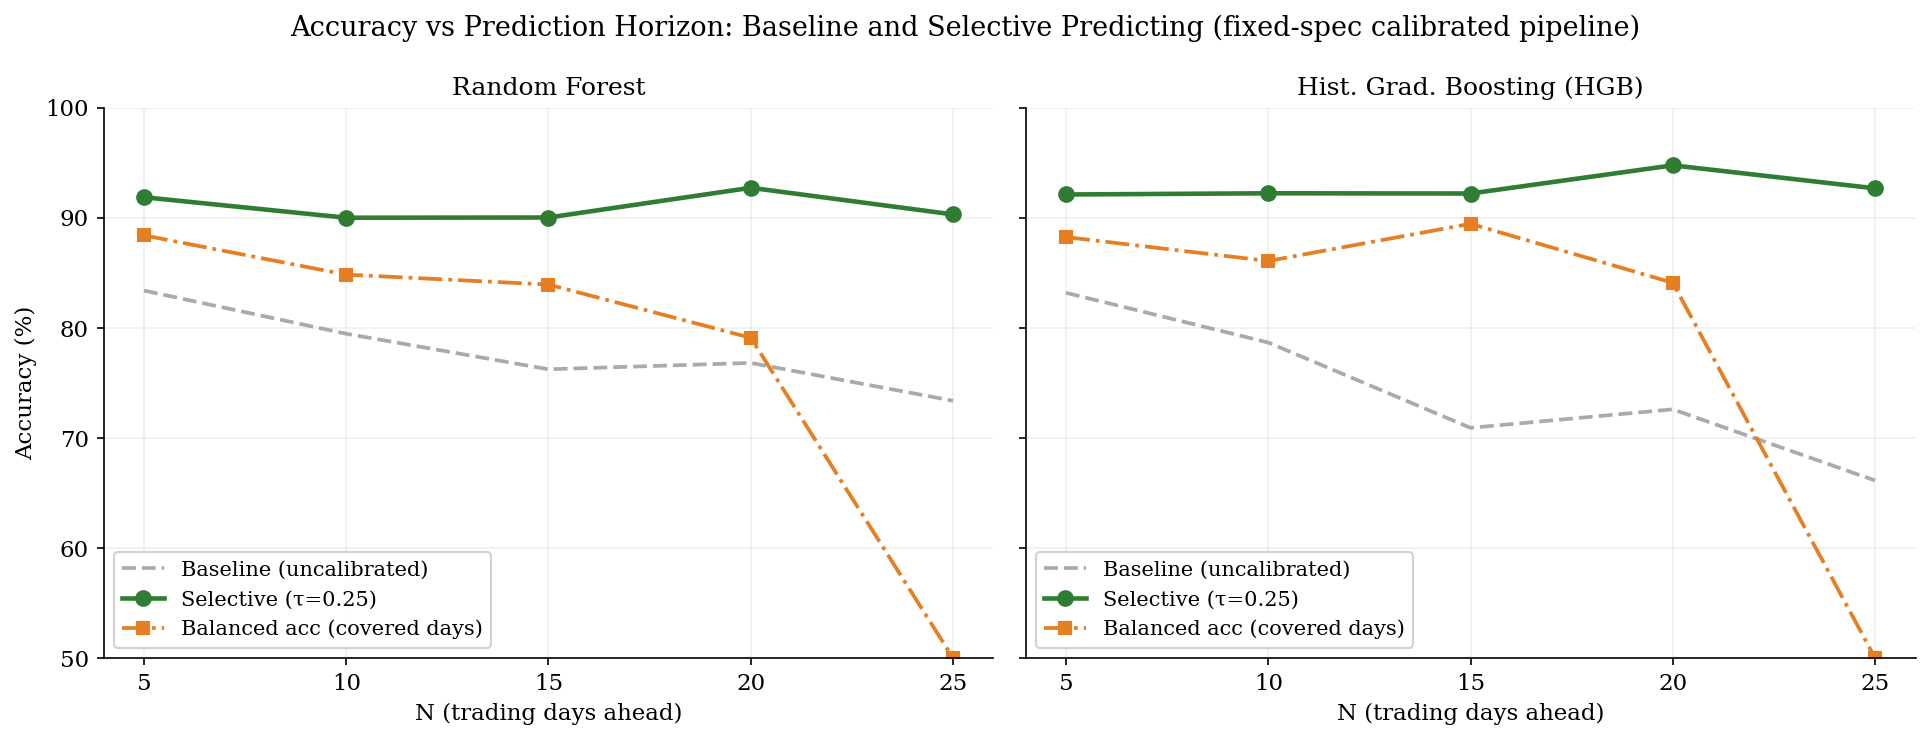
\includegraphics[width=0.85\textwidth]{tuned_model_comparison.png}
    \caption{Baseline, selective accuracy, and balanced accuracy across prediction horizons for Random Forest (left) and HGB (right). Selective accuracy (green) remains high across horizons while baseline accuracy (gray dashed) declines. Balanced accuracy (orange) reveals the class-imbalance artifact: at $N = 25$, balanced accuracy equals 50\%, confirming a coin-flip result despite 90\% selective accuracy.}
    \label{fig:main}
\end{figure}

Selective prediction improves accuracy for both models at every horizon. However, the balanced accuracy columns tell a different story: RF balanced accuracy declines monotonically from 88.4\% at $N = 5$ to 79.1\% at $N = 20$, and collapses to 50.0\% at $N = 25$. This 50\% balanced accuracy at $N = 25$ confirms that the model exclusively predicts low-volatility outcomes on covered days at the longest horizon---a result confirmed by the extended metrics in Table~\ref{tab:extended}, where precision and recall are both 0\% for the positive class. HGB exhibits the same degeneracy (HGB BalAcc = 50.0\% at $N = 25$). The nominal 90\%--92\% selective accuracy at $N = 25$ for both models reflects the 70\% base rate of calm days, not predictive skill. As the balanced accuracy columns make clear, $N \leq 20$ represents the practically informative prediction window.

At $N = 20$, precision reaches 100\% (no false positive spike warnings on covered days) but recall falls to 58\% (42\% of actual spikes missed). This precision-recall tradeoff is characteristic of a model that abstains on uncertain days: the covered days are predominantly clear-cut, while the borderline transition days (most likely to be spikes) fall in the abstention zone.

\subsection{Threshold Sensitivity}

Table~\ref{tab:threshold} and Figure~\ref{fig:threshold} show RF selective accuracy and coverage across confidence thresholds for $N = 5$ and $N = 10$.

\begin{table}[H]
\centering
\caption{Random Forest selective accuracy and coverage as a function of confidence threshold $\tau$ (fixed-spec calibrated pipeline).}
\label{tab:threshold}
\begin{tabular}{ccccc}
\toprule
$\tau$ & RF $N{=}5$ Acc & $N{=}5$ Cov & RF $N{=}10$ Acc & $N{=}10$ Cov \\
\midrule
0.10 & 86.5\% & 91.0\% & 83.3\% & 90.5\% \\
0.15 & 88.3\% & 85.1\% & 84.7\% & 85.9\% \\
0.20 & 89.0\% & 82.9\% & 86.6\% & 78.5\% \\
0.25 & 91.9\% & 76.3\% & 90.0\% & 60.1\% \\
0.30 & 92.3\% & 73.6\% & 91.8\% & 53.6\% \\
0.35 & 95.0\% & 67.1\% & 95.1\% & 36.5\% \\
0.40 & 97.4\% & 49.0\% & 97.4\% & 15.3\% \\
\bottomrule
\end{tabular}
\end{table}

\begin{figure}[H]
    \centering
    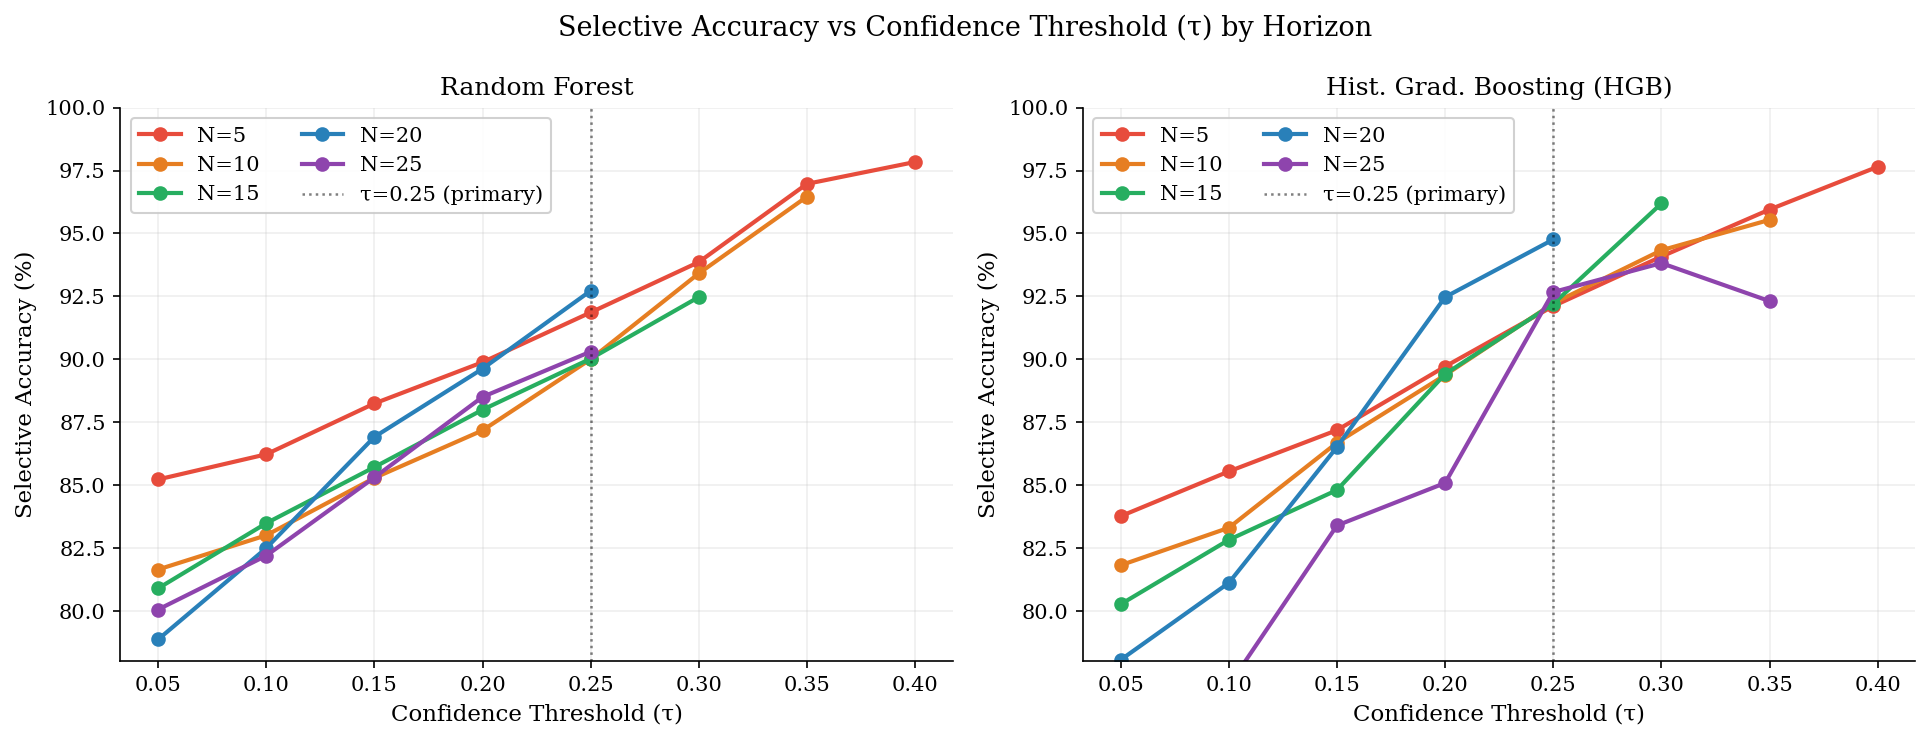
\includegraphics[width=0.75\textwidth]{threshold_optimization.png}
    \caption{Random Forest selective accuracy as a function of confidence threshold $\tau$ for each prediction horizon $N$. Accuracy increases monotonically with $\tau$ across all horizons.}
    \label{fig:threshold}
\end{figure}

Accuracy increases monotonically with $\tau$ across all horizons for the RF. This confirms that the calibrated probability is a reliable ranking signal: predictions at higher confidence levels are systematically more accurate. However, as Section~\ref{sec:transitions} shows, increasing $\tau$ does not improve coverage of transition days---it makes confident wrong predictions on calm$\to$high days even more selective. No choice of $\tau$ converts the framework into a regime-change detector.

\subsection{Robustness Across VIX Thresholds}

\begin{table}[H]
\centering
\caption{Random Forest accuracy gain (selective vs.\ baseline) by VIX regime threshold at $\tau = 0.25$, using the same fixed-spec calibrated pipeline throughout. All gains are positive except RF at $N = 25$ with VIX $\geq$ 18 ($-14.8$\%), where the gain collapses due to the degenerate prediction behavior noted at $N = 25$.}
\label{tab:robust}
\begin{tabular}{cccc}
\toprule
$N$ & VIX $\geq$ 18 & VIX $\geq$ 20 & VIX $\geq$ 22 \\
\midrule
5  & $+$5.4 pp  & $+$8.5 pp  & $+$7.5 pp  \\
10 & $+$11.3 pp & $+$10.5 pp & $+$10.3 pp \\
15 & $+$14.8 pp & $+$13.8 pp & $+$7.9 pp  \\
20 & $+$22.3 pp & $+$15.9 pp & $+$9.1 pp  \\
25 & $-$14.8 pp & $+$16.9 pp & $+$8.3 pp  \\
\bottomrule
\end{tabular}
\end{table}

\begin{figure}[H]
    \centering
    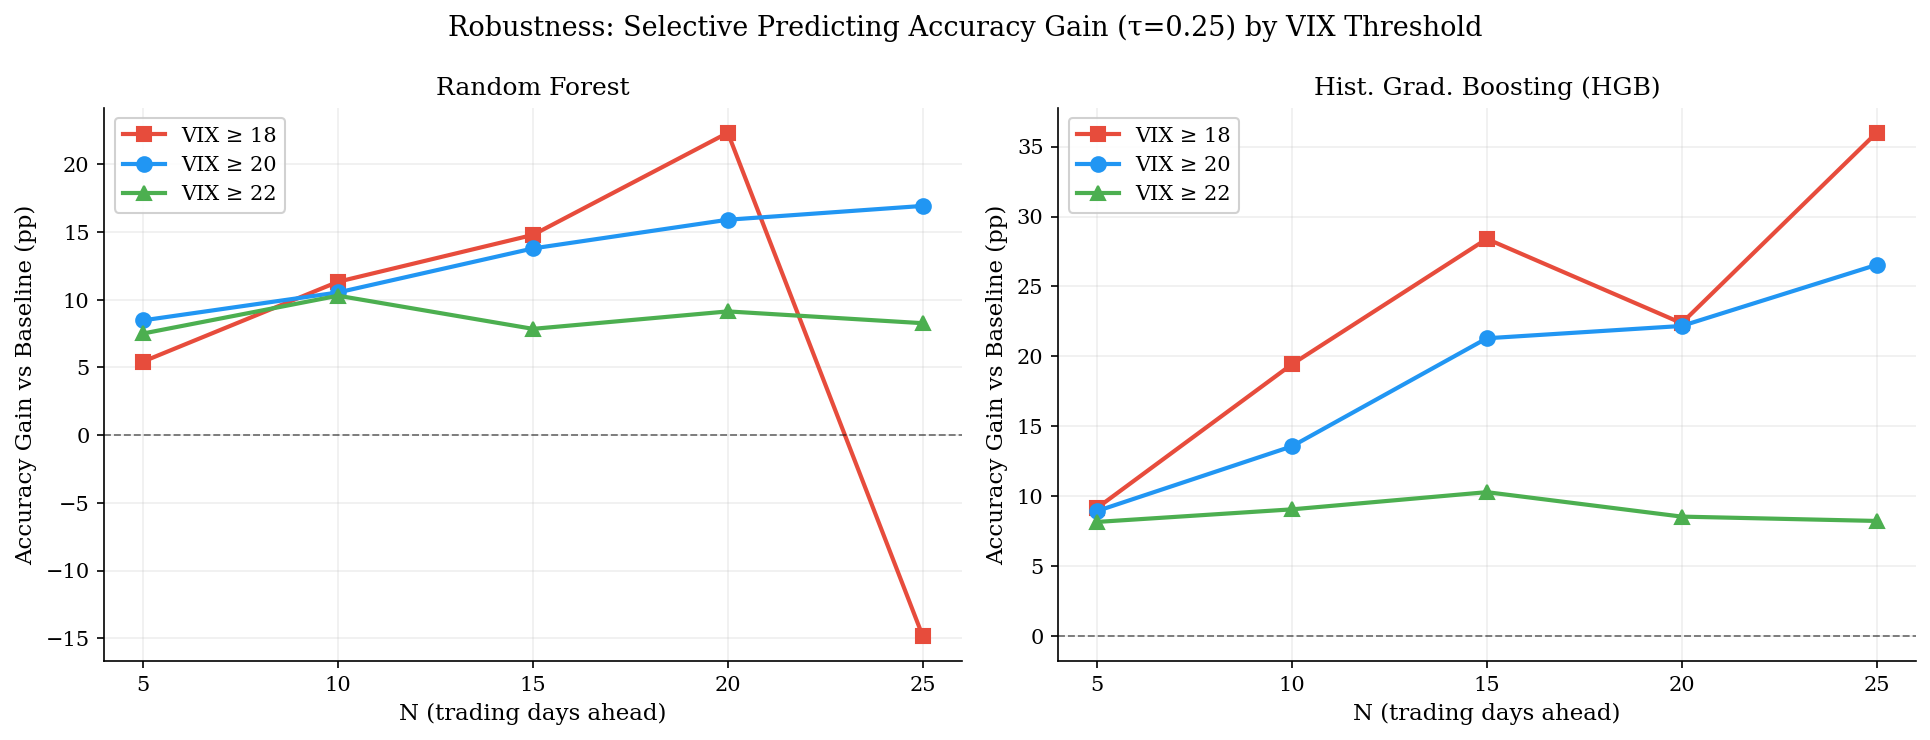
\includegraphics[width=0.75\textwidth]{robustness_check.png}
    \caption{Accuracy gain from selective prediction across VIX thresholds of 18, 20, and 22, plotted against prediction horizon for Random Forest (left) and HGB (right).}
    \label{fig:robust}
\end{figure}

The advantage of selective prediction holds across VIX thresholds of 18, 20, and 22 at $N \leq 20$. The exception is RF at $N = 25$, VIX $\geq$ 18, which shows a gain of $-14.8$ pp. This collapse is consistent with the degenerate behavior documented in Table~\ref{tab:extended}: at the longest horizon with the most inclusive threshold, the model's selective predictions are entirely one-class (calm), yielding accuracy below the corresponding baseline.

\subsection{Sustained Regime Labels}
\label{sec:sustained}

\begin{table}[H]
\centering
\caption{Random Forest selective accuracy for instantaneous and sustained regime labels at $\tau = 0.25$.}
\label{tab:sustained}
\begin{tabular}{ccc}
\toprule
$N$ & Instantaneous & Sustained \\
\midrule
5  & 91.9\% & 94.0\% \\
10 & 90.0\% & 93.8\% \\
15 & 90.0\% & 93.8\% \\
20 & 92.7\% & 94.3\% \\
25 & 90.3\% & 89.9\% \\
\bottomrule
\end{tabular}
\end{table}

Sustained regime labels are consistently easier to predict than instantaneous labels at horizons $N \leq 20$. Persistent high-volatility episodes tend to be preceded by stronger and more consistent signals across multiple features, whereas single-day VIX threshold crossings can be driven by idiosyncratic shocks with little advance warning. At $N = 25$, the sustained label requires VIX to stay at or above 20 for all 25 consecutive days---an increasingly rare event at longer horizons---leaving very few positive examples in the test set; the slight reversal (sustained 89.9\% vs.\ instantaneous 90.3\%) reflects this positive-class scarcity rather than a genuine change in model behavior.

\subsection{Comparison to Naive Baselines}
\label{sec:baselines}

A critical question is whether the RF selective accuracy reflects genuine multi-feature ML skill or simply VIX autocorrelation. To answer this, we construct four coverage-matched baselines plus an uncovered reference predictor, all evaluated on the same test set.

The \textbf{persistence baseline} predicts $\text{VIX}_{t+N} \geq 20$ if and only if $\text{VIX}_t \geq 20$, and abstains when $|\text{VIX}_t - 20| < c$ for a constant $c$ chosen to match the RF's coverage. The \textbf{LR (VIX only) baseline} applies the full calibration pipeline to a single feature (current VIX level). The \textbf{HAR-style logistic regression} uses three features motivated by the HAR model \citep{corsi2009}: current VIX ($\text{VIX}_D$), 5-day VIX mean ($\text{VIX}_W$), and 20-day VIX mean ($\text{VIX}_M$). The \textbf{Markov-chain baseline} estimates the 1-step transition probability matrix from training data and raises it to the $N$th power to predict the probability of being in a high-volatility regime $N$ days ahead; it represents the classical regime-switching forecast under the assumption that regimes follow a first-order Markov process, and serves as a reference for how much ML models add beyond that structural assumption. An \textbf{always-calm predictor}, which issues a calm prediction on every test day unconditionally, appears in Section~\ref{sec:utility} as a lower bound on cost-weighted utility. All baselines and the RF use the same 80/20 train/test split and are evaluated on identical test sets.

\begin{table}[H]
\centering
\caption{RF selective accuracy vs.\ naive baselines at matched coverage ($\tau = 0.25$). HAR-LR = HAR-style logistic regression on (VIX$_D$, VIX$_W$, VIX$_M$). Bolded cell values indicate where a baseline exceeds the RF selective accuracy. Bootstrap CIs for the RF--persistence gap appear in Table~\ref{tab:boot}.}
\label{tab:baselines}
\begin{tabular}{cccccccc}
\toprule
$N$ & Coverage & Persistence & LR (VIX) & \textbf{HAR-LR} & Markov & RF Sel & RF$-$Persist \\
\midrule
5  & 76.3\% & 91.6\% & 91.8\% & 91.6\% & 83.7\% & 91.9\% & $+$0.3 pp \\
10 & 60.1\% & 88.1\% & 87.6\% & \textbf{91.1\%} & 85.3\% & 90.0\% & $+$1.9 pp \\
15 & 51.3\% & 87.9\% & 88.4\% & \textbf{90.2\%} & 84.8\% & 90.0\% & $+$2.1 pp \\
20 & 31.7\% & 90.5\% & 87.9\% & \textbf{94.2\%} & 84.5\% & 92.7\% & $+$2.3 pp \\
25 & 26.9\% & 83.8\% & 86.8\% & \textbf{92.0\%} & 82.9\% & 90.3\% & $+$6.5 pp \\
\bottomrule
\end{tabular}
\end{table}

\begin{figure}[H]
    \centering
    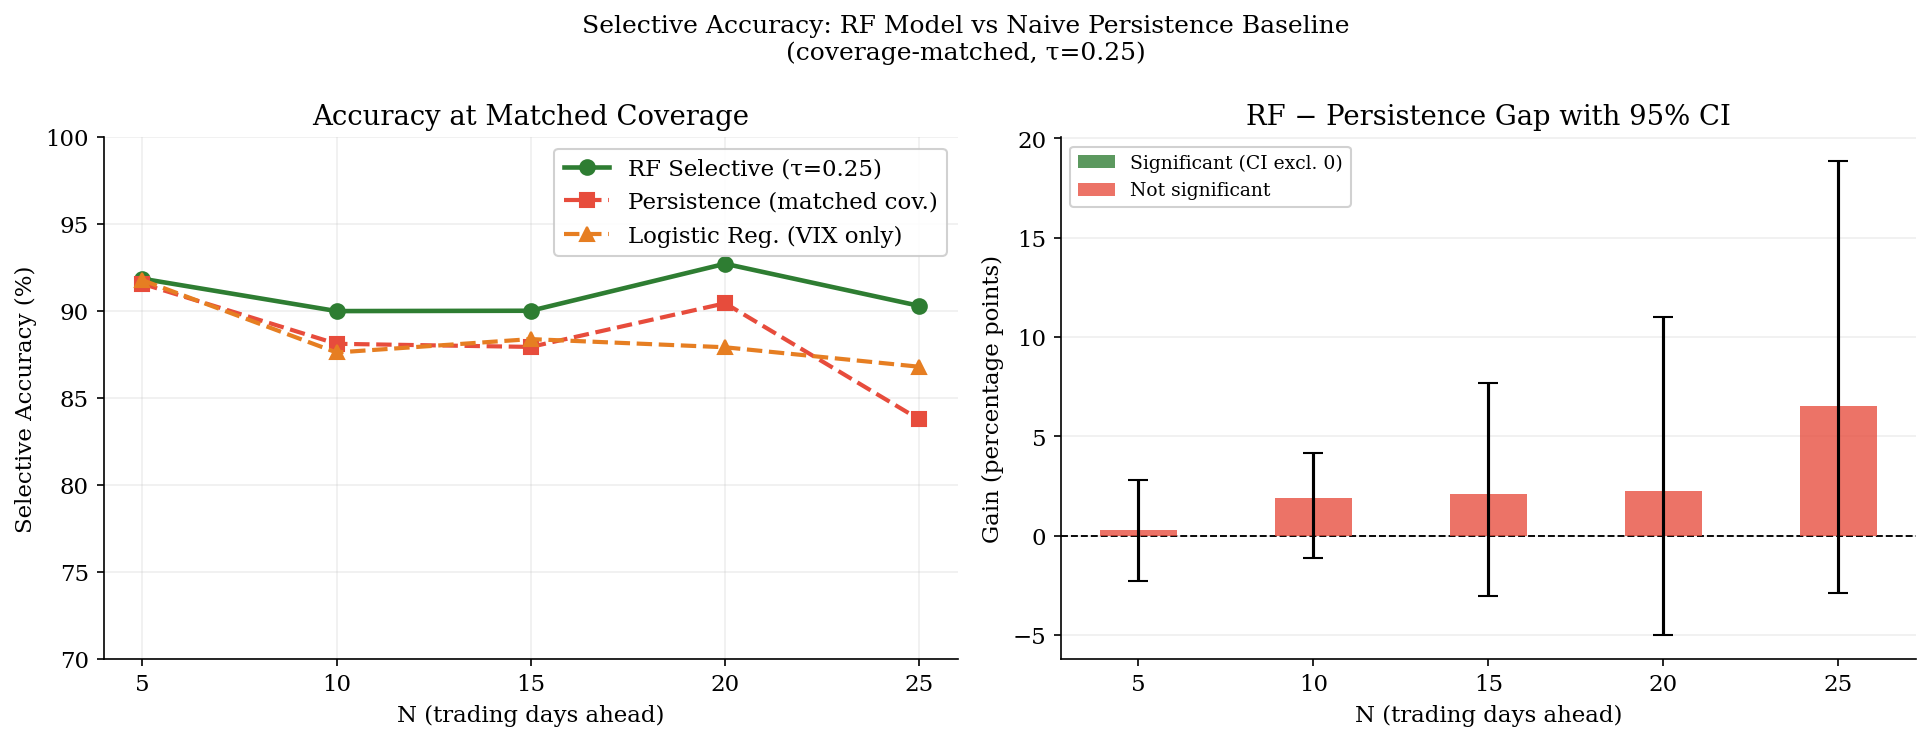
\includegraphics[width=0.85\textwidth]{persistence_baseline.png}
    \caption{Left: RF selective vs.\ naive baseline accuracy at matched coverage across horizons. Right: RF vs.\ persistence gap with 95\% moving-block bootstrap CI. No bar is statistically significant at 5\%.}
    \label{fig:baselines}
\end{figure}

Table~\ref{tab:baselines} delivers the paper's sharpest negative result. The HAR-style logistic regression---using only three VIX-related features---matches or exceeds the full 36-feature RF in point estimate at four of five horizons ($N = 10$, 15, 20, and 25). At $N = 10$, HAR-LR achieves 91.1\% vs.\ the RF's 90.0\%; at $N = 20$, 94.2\% vs.\ 92.7\%. A moving-block bootstrap on the HAR-minus-RF gap at $N = 10$ (HAR leads by $+1.1$ pp) yields 95\% CI $[-1.08, +4.18]$; the corresponding RF-minus-persistence bootstrap gives CI $[-1.11, +4.17]$. Neither gap is statistically confirmed. The 33 additional features (equity, cross-asset, macro) contribute negligibly beyond the three-variable VIX autoregressive structure.

At $N = 5$, the RF selective (91.9\%), HAR-LR (91.6\%), LR-VIX (91.8\%), and persistence (91.6\%) are all essentially identical, confirming that the short-horizon signal is entirely VIX autocorrelation. Notably, the single-feature LR-VIX (91.8\%) marginally outperforms the three-feature HAR-LR (91.6\%) at this horizon, suggesting that adding the weekly and monthly VIX means provides no benefit at $N = 5$.

The RF--persistence gap ($+0.3$ to $+6.5$ pp) is directionally consistent but as Section~\ref{sec:bootstrap} shows, none reaches statistical significance. The $N = 25$ gap ($+6.5$ pp) should be discounted because the RF at this horizon exclusively predicts calm outcomes (Table~\ref{tab:extended}), inflating its nominal accuracy via the class-imbalance base rate; HAR-LR at $N = 25$ (92.0\%) achieves a higher figure, though its behavior at this degenerate horizon is similarly difficult to interpret without extended metrics.

\subsection{Regime Transition Analysis}
\label{sec:transitions}

The selective prediction rule abstains when the model is uncertain; understanding \emph{which days} it covers reveals the economic content of the confidence filter. We classify each test day by the regime at time $t$ and the realized regime at $t + N$, creating four transition categories: calm$\to$calm, calm$\to$high, high$\to$calm, and high$\to$high.

\begin{table}[H]
\centering
\caption{RF selective coverage and accuracy by regime transition type ($\tau = 0.25$, test set). Coverage = fraction of days in that transition category where the model makes a prediction. Accuracy = correctness on covered days only. Calm$\to$high accuracy is \textbf{0\%}: every covered prediction on a day about to spike is a confident ``stay calm'' signal.}
\label{tab:trans}
\begin{tabular}{lcccccc}
\toprule
Transition & \multicolumn{3}{c}{$N = 5$} & \multicolumn{3}{c}{$N = 10$} \\
\cmidrule(lr){2-4}\cmidrule(lr){5-7}
           & Days & Coverage & Acc (covered) & Days & Coverage & Acc (covered) \\
\midrule
calm $\to$ calm & 614 & 87.1\% & 99.6\% & 587 & 71.6\% & 100.0\% \\
calm $\to$ high &  79 & 45.6\% & \textbf{0.0\%}   & 101 & 41.6\% & \textbf{0.0\%} \\
high $\to$ calm &  84 & 35.7\% & 23.3\%         & 111 & 18.0\% & 10.0\% \\
high $\to$ high & 222 & 72.5\% & 99.4\%         & 199 & 59.3\% & 100.0\% \\
\bottomrule
\end{tabular}
\end{table}

\begin{figure}[H]
    \centering
    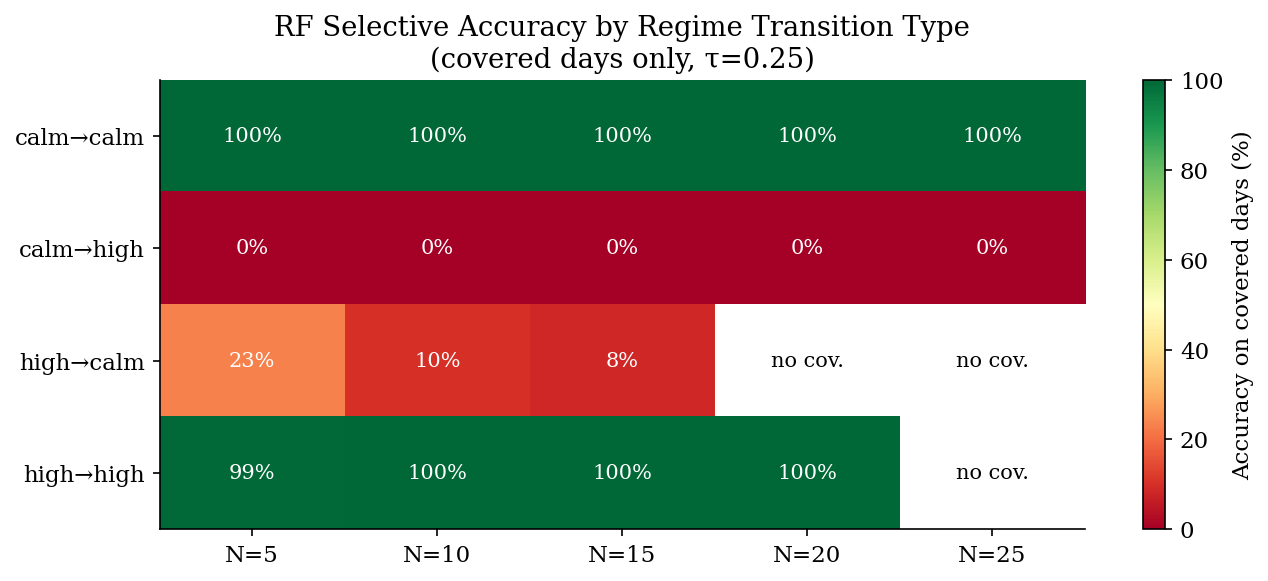
\includegraphics[width=0.65\textwidth]{transition_analysis.png}
    \caption{RF selective accuracy by regime transition type and horizon (covered days only, $\tau = 0.25$). Green = high accuracy; red = low. Calm$\to$high rows are uniformly red at all horizons.}
    \label{fig:trans}
\end{figure}

The table reveals the fundamental limitation of the framework. At $N = 5$, the model covers 36 of 79 calm$\to$high days (45.6\%). On \emph{every single one} of those 36 days, it issues a confident ``stay calm'' prediction---and is wrong. The mechanism is clear: VIX comfortably below 20 generates calibrated probabilities below 0.25, triggering a high-confidence calm prediction. The model is correct that such days usually remain calm, but on the minority of cases where a spike follows, it is confidently mistaken.

\paragraph{Structural caveat.}
This failure is not a model-specific defect: it is an expected property of the prediction problem. Calm$\to$high transitions are disproportionately triggered by exogenous events---geopolitical shocks, central bank surprises, sudden liquidity dislocations, pandemic-scale disruptions---whose onset leaves no advance signature in publicly available daily price and macro features. A model built on such features is analogous to a thermometer used as an earthquake predictor: it measures something real, performs well under normal conditions, but is structurally blind to the shock class because the information simply is not in the instrument. The diagnostic value of 0\% covered accuracy is therefore not that the model is badly calibrated, but that the confidence filter fails to surface its own ignorance---issuing confident wrong predictions on covered transition days rather than abstaining. An early-warning application would require either features that carry event-anticipation content (options skew, credit spreads, order-flow imbalance) or a fundamentally different modeling target.

The aggregate accuracy figures (89--92\%) are therefore driven almost entirely by the two diagonal cells (calm$\to$calm and high$\to$high), which together account for over 80\% of test days. The off-diagonal cells both show poor accuracy: calm$\to$high covered accuracy is 0\%, while high$\to$calm covered accuracy is 23.3\% at $N = 5$ and 10.0\% at $N = 10$---both substantially below the 50\% random baseline. On days when VIX is elevated but will revert to calm within $N$ days, the model confidently predicts continued high volatility and is wrong more often than chance. A practitioner using this framework as a spike early-warning system would receive confident, wrong ``all clear'' signals on nearly half of the days before a spike materialized.

\paragraph{Cost-weighting does not rescue calm$\to$high recall.}
To test whether the 0\% calm$\to$high covered accuracy reflects an objective-function deficiency rather than an information ceiling, we refit the RF with explicit class weights $\{0{:}1, 1{:}w\}$ for $w \in \{1, 5, 10, 20\}$, penalizing false negatives on high-volatility days by up to 20$\times$ relative to false positives. At $N = 5$, calm$\to$high day coverage increases modestly from 45.6\% to 49.4\% as $w$ rises, but covered accuracy remains \textbf{0.0\% at every weight}. At $N = 10$, calm$\to$high coverage increases more substantially from 41.6\% to 58.4\% under $w = 10$, yet every covered prediction is still a confident ``stay calm.'' The coverage increase under heavy weighting is not paradoxical: aggressive class-weighting pushes the RF to assign higher probabilities to the days it classifies as high-vol; the subsequent isotonic calibration then maps the remaining days---including calm$\to$high transitions, which are feature-indistinguishable from ordinary calm days---to even lower calibrated probabilities, pushing more of them below $0.5 - \tau$ and into the high-confidence calm zone rather than the abstention zone. Cost-weighted utility also worsens monotonically with $w$: at $N = 10$, the unweighted RF achieves utility $-0.730$ under cost ratio $C = 10$ (Table~\ref{tab:utility}), and increasing the class weight strictly worsens this figure at every cost ratio tested. The class-weighting experiment delivers a clean verdict: the failure to predict calm$\to$high transitions is \emph{informational}, not objective-function-driven. The daily feature set does not contain enough advance information about shock onset to produce correct predictions on transition days regardless of how heavily the training objective penalizes misses.

\begin{table}[H]
\centering
\caption{Effect of class-weighting on transition coverage and selective accuracy. $w$ = false-negative class weight; $\tau = 0.25$ throughout. C$\to$H = calm$\to$high; C$\to$C = calm$\to$calm. Calm$\to$high accuracy is \textbf{0.0\%} at every weight for both horizons.}
\label{tab:reweight}
\begin{tabular}{ccrrcrc}
\toprule
$N$ & $w$ & C$\to$H Cov & C$\to$H Acc & C$\to$C Cov & C$\to$C Acc & Sel Acc \\
\midrule
5 &  1 & 45.6\% & \textbf{0.0\%} & 87.1\% & 99.6\%  & 91.9\% \\
5 &  5 & 46.8\% & \textbf{0.0\%} & 87.1\% & 100.0\% & 92.2\% \\
5 & 10 & 49.4\% & \textbf{0.0\%} & 87.3\% & 100.0\% & 92.3\% \\
5 & 20 & 48.1\% & \textbf{0.0\%} & 84.4\% & 100.0\% & 91.8\% \\
\midrule
10 &  1 & 41.6\% & \textbf{0.0\%} & 71.6\% & 100.0\% & 90.0\% \\
10 &  5 & 49.5\% & \textbf{0.0\%} & 77.7\% & 100.0\% & 89.5\% \\
10 & 10 & 58.4\% & \textbf{0.0\%} & 80.4\% & 100.0\% & 87.4\% \\
10 & 20 & 57.4\% & \textbf{0.0\%} & 82.8\% & 100.0\% & 87.4\% \\
\bottomrule
\end{tabular}
\end{table}

\paragraph{Abstention as a leading indicator.} The transition analysis reveals a subtler and more positive finding. Although the model cannot make correct \emph{predictions} on calm$\to$high days, we test whether its \emph{abstention rate} is elevated in the days leading up to such transitions.

\begin{figure}[H]
    \centering
    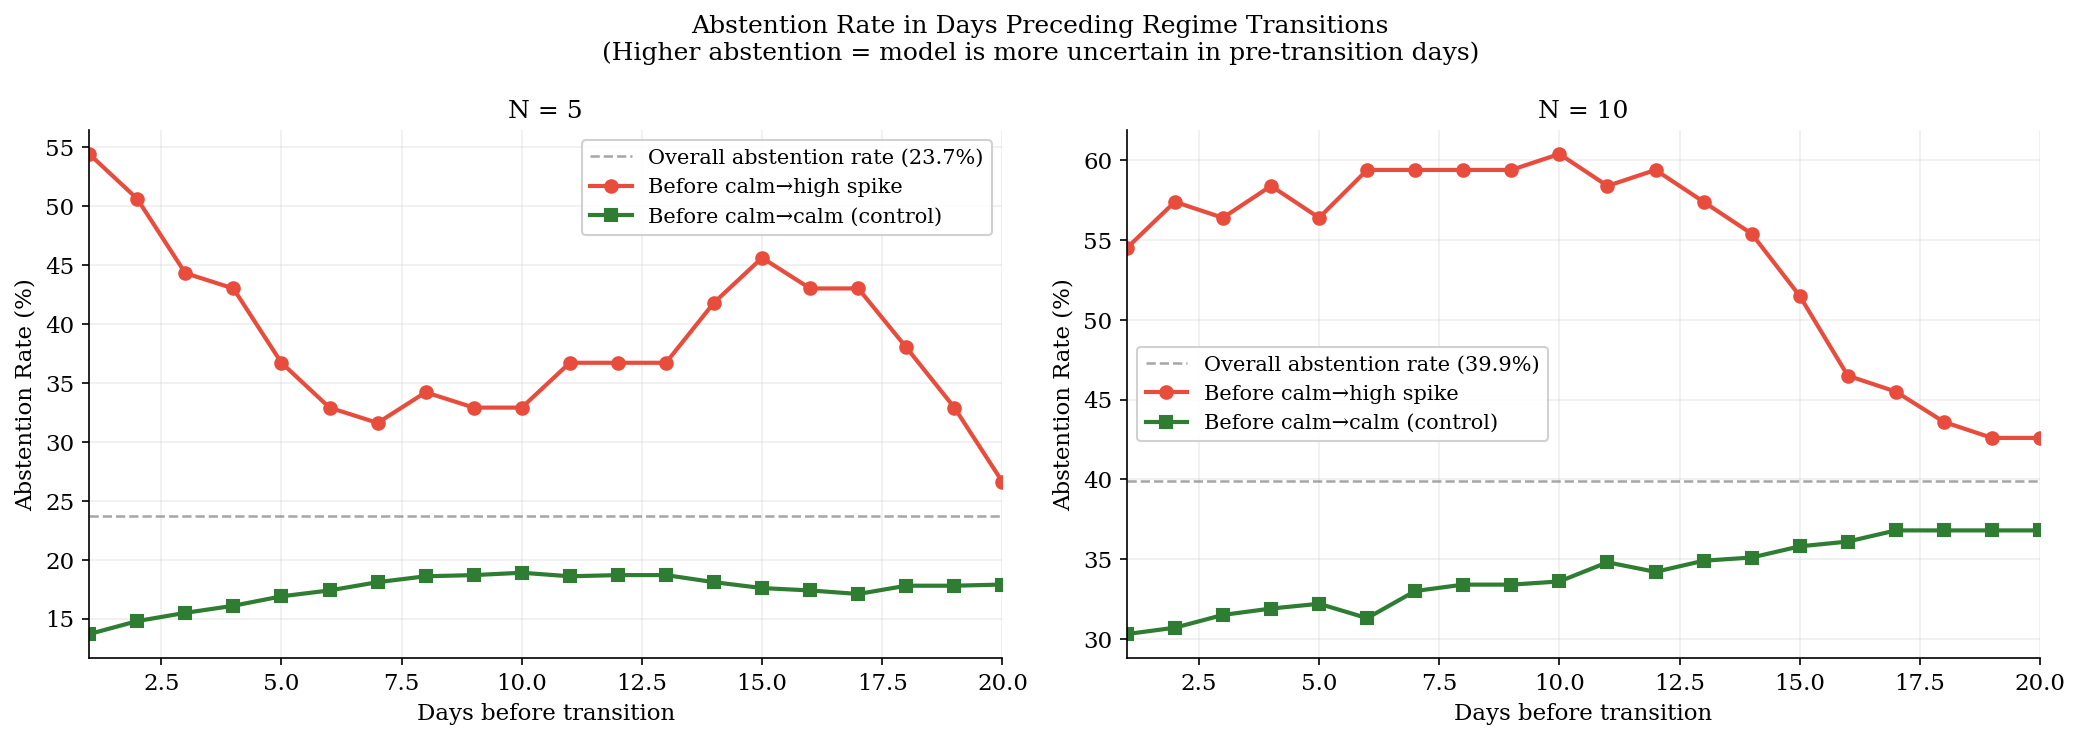
\includegraphics[width=0.85\textwidth]{abstention_analysis.png}
    \caption{Abstention rate in the days preceding calm$\to$high transitions (red) vs.\ calm$\to$calm days (green), compared to the overall abstention rate (dashed). At lag = 1 day, the abstention rate before spikes is more than double the overall rate.}
    \label{fig:abstention}
\end{figure}

Figure~\ref{fig:abstention} shows that at $N = 5$, the abstention rate in the day immediately before a calm$\to$high transition is 54.4\%, compared to 13.7\% before calm$\to$calm days and 23.7\% overall---a 2.3$\times$ elevation. At $N = 10$, the corresponding rates are 54.5\% vs.\ 30.3\% vs.\ 39.9\% (1.4$\times$). This observation carries a necessary qualification: it is a post-hoc pattern measured on the same held-out test set used for all other results, and should be treated as hypothesis-generating rather than confirmatory.

\paragraph{Confound test: abstention vs.\ VIX proximity.}
A natural concern is that the abstention elevation trivially reflects VIX proximity to the threshold: calm$\to$high transitions start from $\text{VIX}_t < 20$ by definition, and days near the boundary may generate uncertain probabilities simply because the feature distribution near $\text{VIX}_t \approx 20$ is ambiguous. To test this, we compare three signals as binary spike classifiers on calm days only ($\text{VIX}_t < 20$): the raw abstention indicator, the proximity score $1 - (\text{VIX}_t^{\max} - \text{VIX}_t) / (\text{VIX}_t^{\max} - \text{VIX}_t^{\min})$ where the range is taken over calm-day test observations,\footnote{An equivalent range-free formulation is $20 - \text{VIX}_t$ (negated distance), which yields the same ranking without depending on the test-set min/max. We use the normalized form for AUC comparability with the probability scores.} and the HAR-LR calibrated probability. We evaluate each with ROC/AUC and apply a moving-block bootstrap (2,000 replicates, block length $\approx 32$, matching Section~\ref{sec:bootstrap}) to the abstention-rate gap.

\begin{figure}[H]
    \centering
    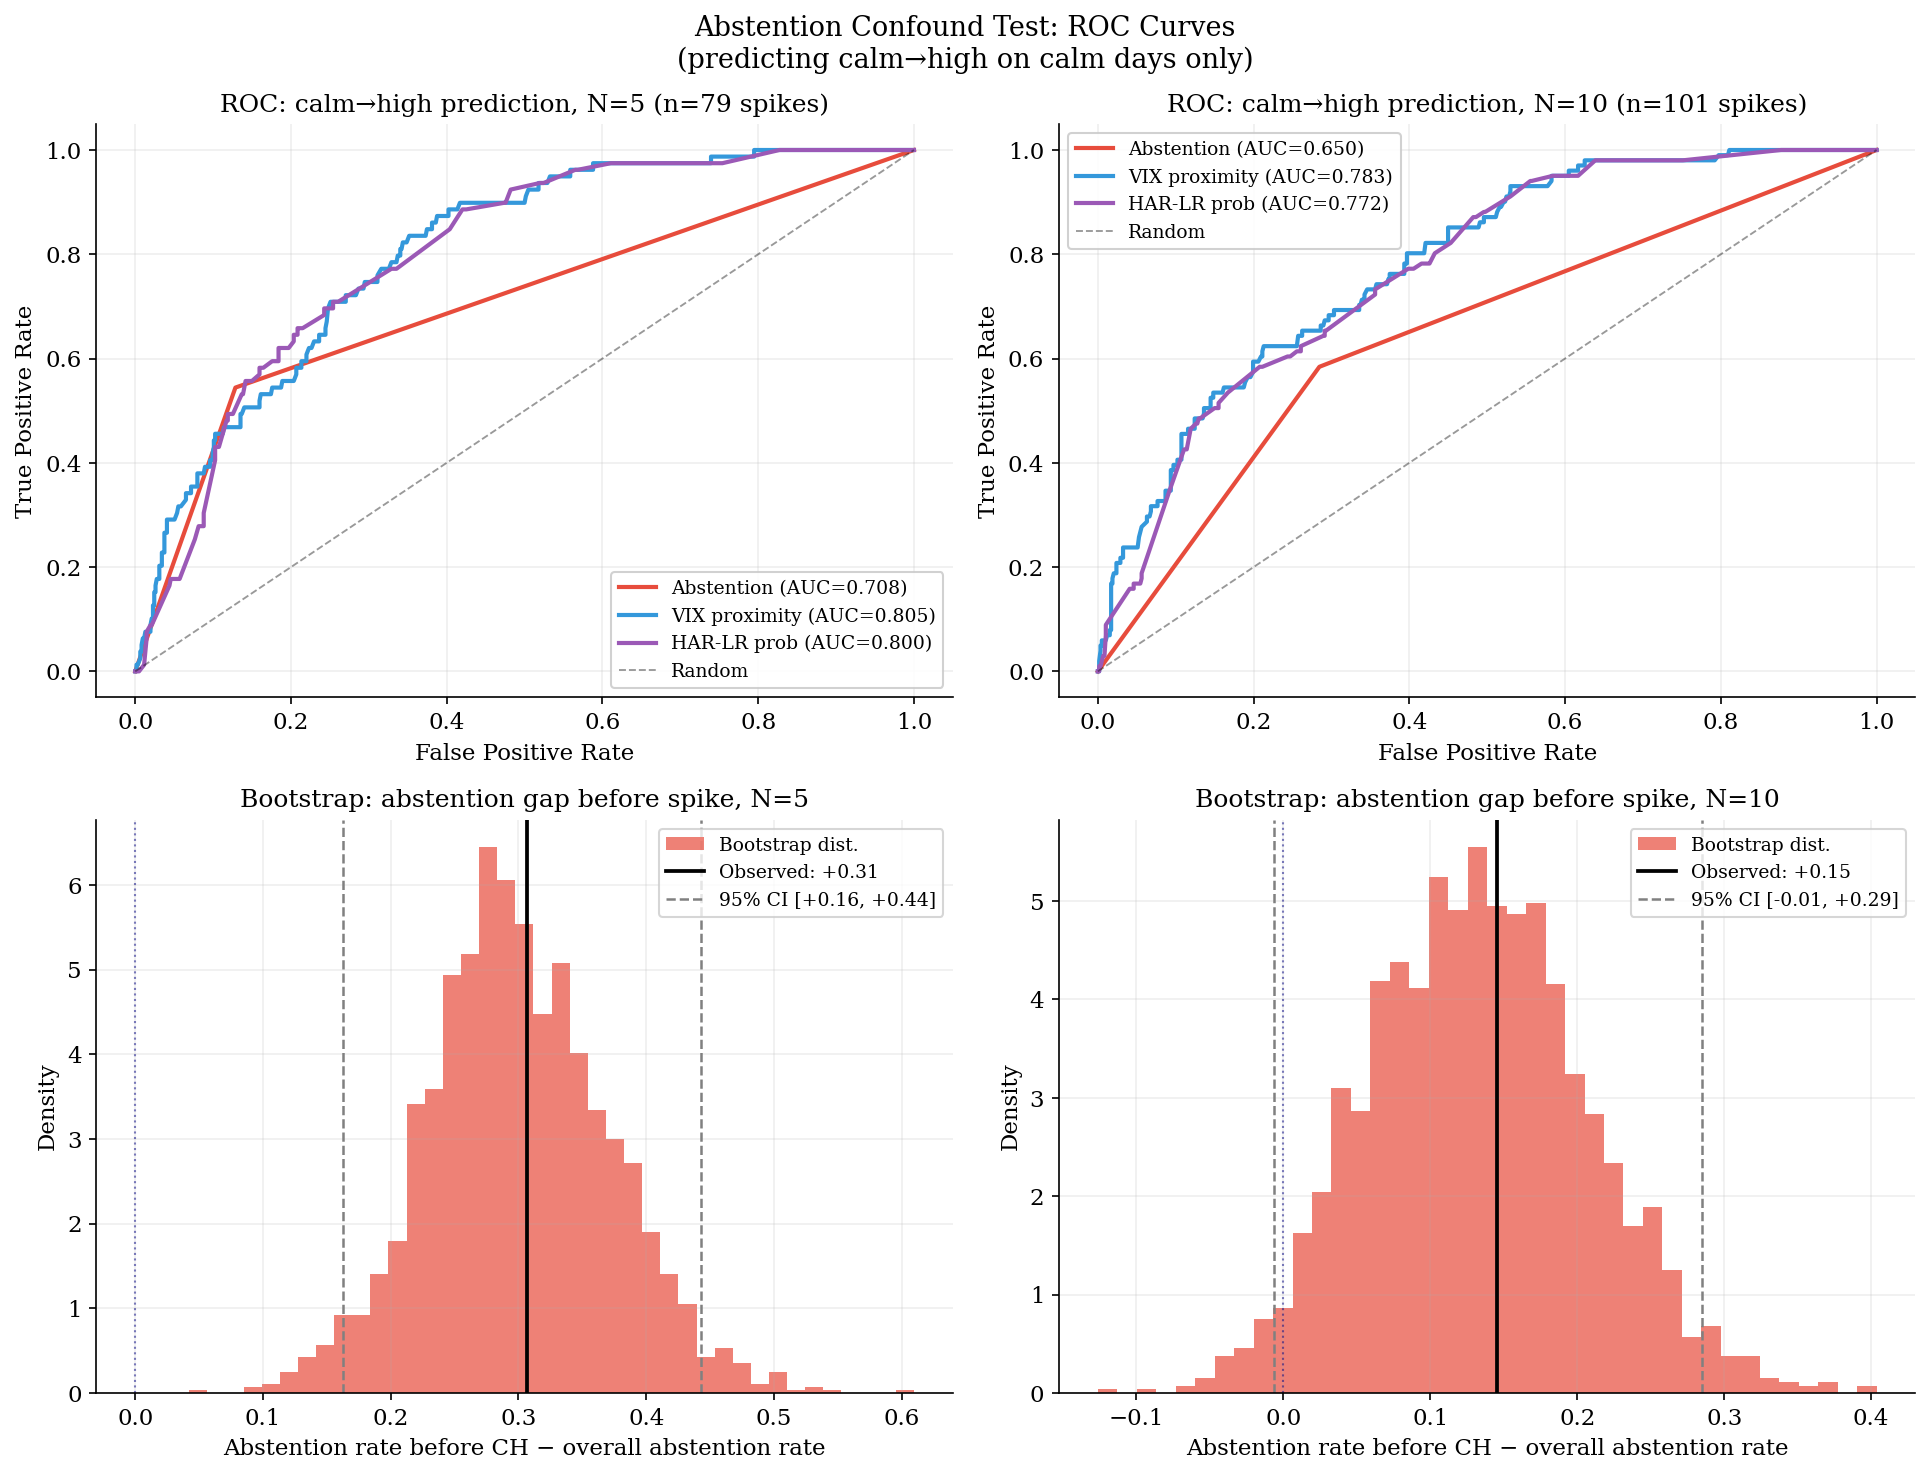
\includegraphics[width=0.85\textwidth]{abstention_confound.png}
    \caption{Top: ROC curves comparing abstention, VIX proximity to threshold, and HAR-LR probability as calm$\to$high predictors on calm days ($\text{VIX}_t < 20$), for $N = 5$ (left) and $N = 10$ (right). Bottom: Moving-block bootstrap distribution of the abstention-rate gap (before calm$\to$high events minus overall rate), with 95\% CI.}
    \label{fig:confound}
\end{figure}

Figure~\ref{fig:confound} (top panels) shows that VIX proximity (AUC $= 0.805$ at $N = 5$; $0.783$ at $N = 10$) and HAR-LR probability (AUC $= 0.800$; $0.772$) both outperform raw abstention (AUC $= 0.708$; $0.650$) as spike classifiers on calm days. The majority of the abstention signal is therefore accounted for by VIX proximity to the threshold.

To test whether abstention carries \emph{incremental} information beyond proximity, we fit two logistic regressions on calm days: one using proximity alone and one using proximity plus the abstention indicator. At $N = 5$, the combined model (AUC $= 0.816$) beats proximity alone (AUC $= 0.805$); the likelihood-ratio statistic on the evaluation data corresponds to $p = 0.001$. However, because the test set was used for all other evaluations in this paper and was not reserved for this test, the $p$-value does not constitute a valid significance claim---it is a descriptive measure of fit improvement on this sample, not a confirmatory finding, and should be treated accordingly. At $N = 10$, the combined model adds nothing (AUC $= 0.782$ vs.\ $0.783$, $p = 1.000$). We treat the $N = 5$ increment as a provisional regularity warranting dedicated out-of-sample confirmation. Abstention therefore carries a small residual signal beyond threshold proximity at the shorter horizon only.

The bootstrap confidence intervals on the abstention-rate gap are: $N = 5$: $+0.307$, 95\% CI $[+0.162, +0.443]$ (significant); $N = 10$: $+0.146$, 95\% CI $[-0.006, +0.285]$ (marginally insignificant). The overall picture is that proximity explains most of the elevation, but at $N = 5$ the model's uncertainty carries a small independent informational increment. We report this as a documented regularity warranting follow-up investigation, not as a robust predictive finding.

\subsection{Walk-Forward Validation}
\label{sec:wf}

Table~\ref{tab:wf} reports five-fold expanding walk-forward results for $N \in \{5, 10, 20\}$. $N = 15$ is omitted because its behavior falls monotonically between $N = 10$ and $N = 20$; $N = 25$ is omitted because the model degenerates to always predicting calm at that horizon (Section~\ref{sec:main}), making fold-to-fold variance uninformative.

\begin{table}[H]
\centering
\caption{5-fold expanding walk-forward validation results, including persistence at RF-matched coverage. Bold entries indicate where persistence exceeds RF selective accuracy. Shaded rows show that at $N = 20$ the RF/HGB gains collapse with standard deviations exceeding 25 pp; persistence remains stable at $N = 20$ (std 7.7\%).}
\label{tab:wf}
\begin{tabular}{cccccc}
\toprule
Model & $N$ & Mean Baseline & Std & Mean Selective & Std \\
\midrule
Random Forest    & 5  & 82.8\% & 9.7\%  & 92.2\% & 1.7\%  \\
Persistence      & 5  & 88.0\% & 3.2\%  & \textbf{93.9\%} & 3.2\%  \\
HGB              & 5  & 84.0\% & 8.0\%  & 84.6\% & 9.7\%  \\
\midrule
Random Forest    & 10 & 72.3\% & 22.7\% & 85.9\% & 7.7\%  \\
Persistence      & 10 & 84.8\% & 4.5\%  & \textbf{91.3\%} & 4.1\%  \\
HGB              & 10 & 70.9\% & 22.9\% & 77.3\% & 15.2\% \\
\midrule
\rowcolor[gray]{0.9}
Random Forest    & 20 & 67.5\% & 22.8\% & 67.1\% & 28.3\% \\
Persistence      & 20 & 81.5\% & 3.9\%  & \textbf{86.2\%} & 7.7\%  \\
\rowcolor[gray]{0.9}
HGB              & 20 & 63.6\% & 25.2\% & 61.4\% & 29.9\% \\
\bottomrule
\end{tabular}
\end{table}

\begin{figure}[H]
    \centering
    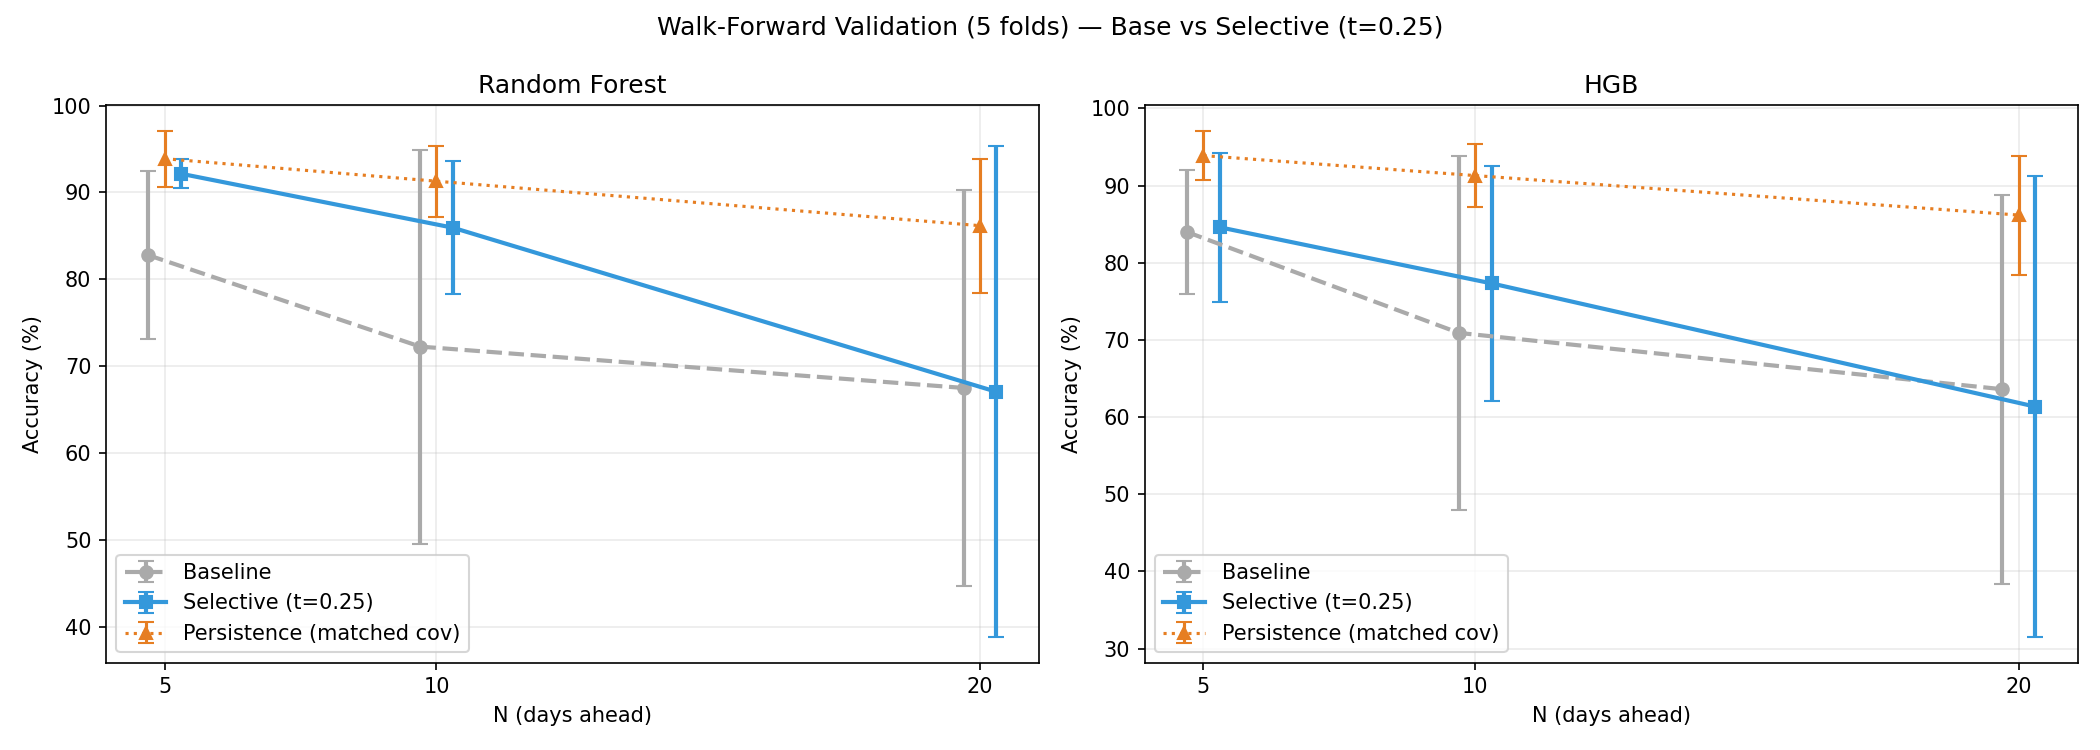
\includegraphics[width=0.75\textwidth]{walk_forward.png}
    \caption{Walk-forward validation results with error bars ($\pm$1 std) for baseline, selective prediction, and coverage-matched persistence (orange) across $N \in \{5, 10, 20\}$ for Random Forest (left) and HGB (right). Persistence matches or exceeds RF selective at all horizons.}
    \label{fig:wf}
\end{figure}

For Random Forest at $N = 5$, selective prediction achieves a mean out-of-sample accuracy of 92.2\% with a standard deviation of only 1.7\% across five folds. The confidence filter makes predictions highly stable across market cycles. However, this result must be shared with the naive baseline: coverage-matched persistence at $N = 5$ achieves 93.9\% $\pm$ 3.2\%---a higher mean than RF with roughly double the fold-to-fold variance. The RF's distinctive property at $N = 5$ is therefore its stability, not a unique accuracy advantage over the naive rule.

At $N = 10$, persistence (91.3\% $\pm$ 4.1\%) exceeds RF selective (85.9\% $\pm$ 7.7\%) in both mean accuracy and stability. Persistence also remains well-behaved at $N = 20$ (86.2\% $\pm$ 7.7\%), whereas RF collapses to 67.1\% $\pm$ 28.3\%.

HGB's walk-forward gain at $N = 5$ is only 0.6 pp (84.6\% vs.\ 84.0\%) with a standard deviation of 9.7\%---negligible compared to RF's 9.4 pp gain and far below persistence's 5.9 pp gain at the same horizon. HGB is retained in the main tables for completeness but offers no practical advantage over RF in the walk-forward evaluation.

At $N = 20$, both RF and HGB show fold-to-fold standard deviations exceeding 25 pp; these results are uninformative rather than negative, and persistence remains stable. The practical reliable prediction window is approximately $N \leq 10$, and within that window, persistence is a formidable competing benchmark.

\subsection{Probability Calibration Quality}
\label{sec:calibration}

Section~\ref{sec:methodology} motivates isotonic regression calibration; Figure~\ref{fig:cal} verifies it on the test set. Each panel shows the reliability diagram for RF at $N = 5$ and $N = 10$, with Brier scores annotated.

\begin{figure}[H]
    \centering
    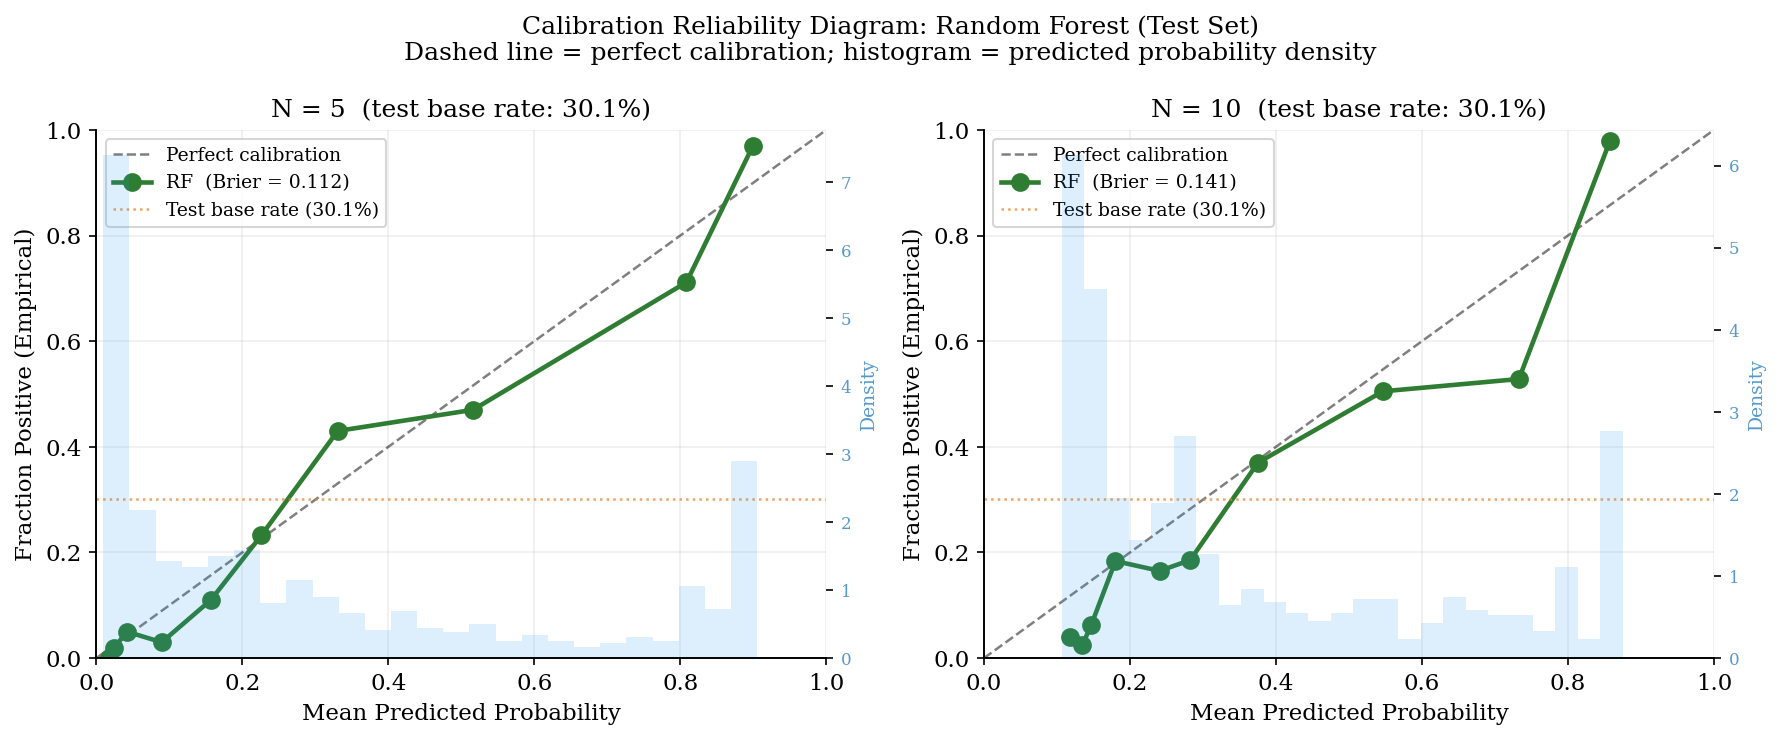
\includegraphics[width=0.85\textwidth]{calibration_diagram.png}
    \caption{Calibration reliability diagrams for RF at $N = 5$ (left) and $N = 10$ (right). Points near the diagonal indicate well-calibrated probabilities. Orange dotted line = test-set base rate ($\approx$30\%).}
    \label{fig:cal}
\end{figure}

Calibrated probabilities are broadly well-ordered on the test set. Brier scores are 0.112 at $N = 5$ and 0.142 at $N = 10$, both well below the no-skill baseline of $\bar{p}(1-\bar{p}) \approx 0.21$ at the test-set base rate of 29.8\%. Calibration is verified at $N = 5$ and $N = 10$ as representative short-horizon cases; $N = 15$ shows qualitatively similar reliability diagrams, and at $N \geq 20$ the model's selective predictions degenerate to always-calm, making full-distribution calibration metrics uninformative. Consistent with the base-rate shift (36.7\% in training, 29.8\% in test), the calibration curve at mid-range probabilities sits slightly above the diagonal, but the monotonic $\tau$-accuracy relationship in Table~\ref{tab:threshold} is preserved.

\subsection{Statistical Significance of the Persistence Gap}
\label{sec:bootstrap}

Section~\ref{sec:baselines} reports an RF vs.\ persistence accuracy gap of $+1.9$ pp at $N = 10$ and $+2.1$--$2.3$ pp at $N = 15$--$20$. To assess statistical significance under serial dependence, we apply a moving-block bootstrap to the paired accuracy difference (RF selective minus persistence, at matched coverage). Block length is set to $\max(\sqrt{N_\text{test}},\, 20) \approx 32$ days following \citet{kunsch1989}; 2,000 bootstrap replicates are drawn; CI endpoints vary by less than 0.1 pp across random seeds.

\begin{table}[H]
\centering
\caption{Moving-block bootstrap 95\% confidence intervals for the RF vs.\ persistence accuracy gap at matched coverage ($\tau = 0.25$). All CIs include 0; no gap is statistically significant at the 5\% level.}
\label{tab:boot}
\begin{tabular}{crrr}
\toprule
$N$ & Gap (pp) & 95\% CI lower & 95\% CI upper \\
\midrule
5  & $+0.30$ & $-2.26$ & $+2.80$ \\
10 & $+1.88$ & $-1.11$ & $+4.17$ \\
15 & $+2.07$ & $-3.03$ & $+7.70$ \\
20 & $+2.28$ & $-5.01$ & $+11.03$ \\
25 & $+6.52$ & $-2.86$ & $+18.87$ \\
\bottomrule
\end{tabular}
\end{table}

\begin{figure}[H]
    \centering
    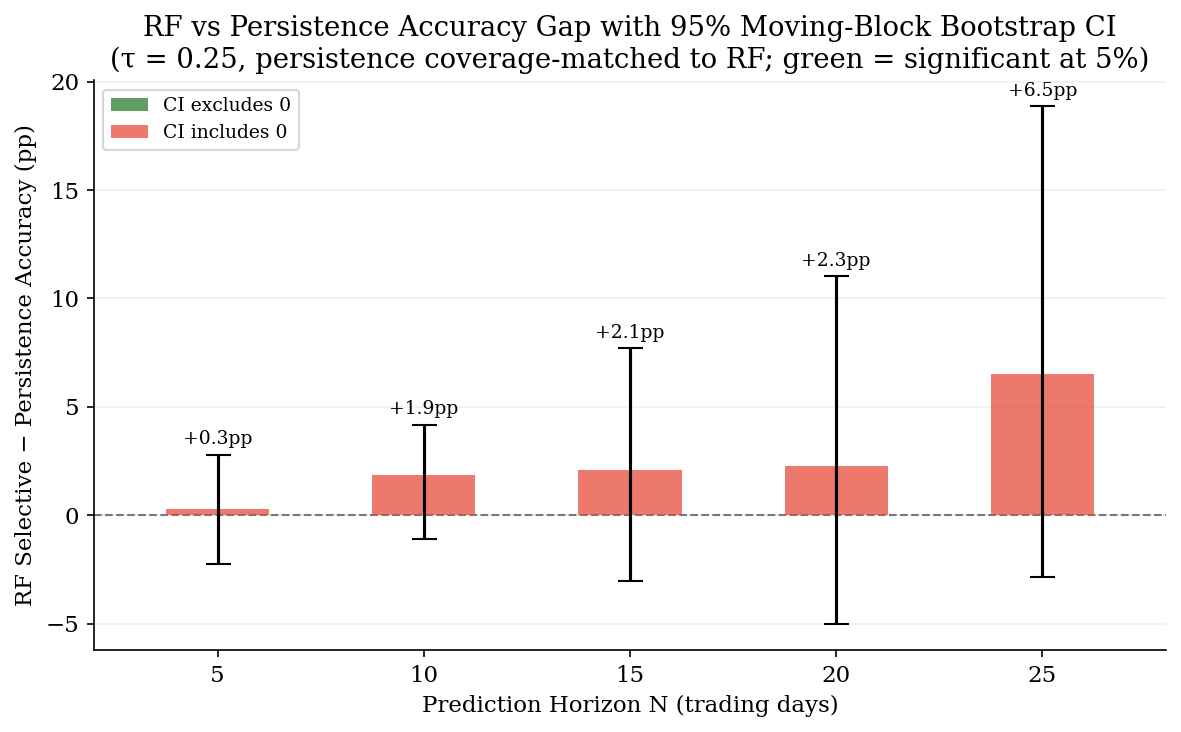
\includegraphics[width=0.70\textwidth]{bootstrap_ci.png}
    \caption{RF vs.\ persistence accuracy gap with 95\% moving-block bootstrap CI. No bar is statistically significant at 5\%; all CIs include 0. $N = 10$ is closest: $+1.88$ pp, CI $[-1.11, +4.17]$.}
    \label{fig:boot}
\end{figure}

No gap is statistically significant at the 5\% level; all confidence intervals include 0. The $N = 10$ result ($+1.88$ pp, 95\% CI $[-1.11, +4.17]$) is the closest to significance. However, the McNemar test below provides a sharper interpretation: because RF and persistence make identical predictions on every jointly covered day at $N \geq 10$, the gaps in Table~\ref{tab:boot} are attributable entirely to differences in \emph{which} days each rule covers, not to differing predictions on shared days. The open question is therefore whether the RF's coverage \emph{selection}---not its predictions---carries independent value; the walk-forward stability at $N = 5$ (RF fold std 1.7\% vs.\ persistence 3.2\%) weakly suggests it might, but the directional accuracy gap does not indicate latent multi-feature predictive skill awaiting more data.

\paragraph{McNemar's test: RF vs.\ persistence on jointly covered days.}
A paired McNemar's test on jointly covered days---days where both the RF selective rule and the coverage-matched persistence rule make a prediction---establishes this composition interpretation precisely. We use the mid-$p$ McNemar variant, which is exact for small $b + c$ and coincides with the chi-squared form when $b + c \geq 25$. At $N = 10$, 15, 20, and 25, the contingency table has $b = c = 0$: RF and persistence make \emph{identical} predictions on every jointly covered day ($\chi^2 = 0$, $p = 1.000$ at all four horizons). At $N = 5$, there are 689 jointly covered days; RF is correct where persistence is wrong on only 3 days ($c = 3$, $b = 0$, gap $= {+}0.44$ pp, $p = 0.083$). The Table~\ref{tab:boot} accuracy gaps are therefore attributable entirely to differences in which days each rule covers, not to differing predictions on shared days. At $N \geq 10$, the RF chooses to make predictions exclusively on days already far from the 20 threshold, producing the same call as the persistence rule on every one of them.

\paragraph{Robustness to 2022 exclusion.}
The year 2022 was an unusually high-volatility period that accounts for 15--17\% of test days depending on horizon. Removing those 149--165 days leaves 830--850 observations per horizon. The qualitative conclusions are unchanged: RF selective still exceeds persistence by $+1.25$ to $+7.34$ pp, HAR-LR matches or beats RF at $N \geq 10$ (HAR leads by $+2.24$ pp at $N = 10$ and $+3.43$ pp at $N = 20$), and calm$\to$high covered accuracy remains 0\% at all horizons. The 2022 bear-market cluster does not explain the paper's primary findings.

\subsection{Permutation Feature Importance}

\begin{table}[H]
\centering
\caption{Top-8 Random Forest features by permutation importance (mean accuracy decrease when feature values are shuffled), averaged across $N \in \{5, 10, 20\}$. Permutation importance avoids the high-cardinality bias of mean decrease in impurity (MDI); the remaining 28 features each cause less than 0.15\% average accuracy drop when shuffled.}
\label{tab:fi}
\begin{tabular}{clcc}
\toprule
Rank & Feature & Avg.\ Importance & Category \\
\midrule
1 & VIX\_SMA10         & 1.88\% & VIX trend \\
2 & SP500\_DRAWDOWN    & 1.08\% & Equity risk \\
3 & VIX\_BB\_LOWER     & 0.52\% & VIX Bollinger bands \\
4 & SP500\_MOM10       & 0.46\% & Equity momentum \\
5 & SP500\_RVOL        & 0.31\% & Realized volatility \\
6 & SP500\_RET20       & 0.27\% & Equity return \\
7 & VIX\_BB\_POSITION  & 0.19\% & VIX Bollinger bands \\
8 & VIX\_ROC20         & 0.18\% & VIX momentum \\
\bottomrule
\end{tabular}
\end{table}

\begin{figure}[H]
    \centering
    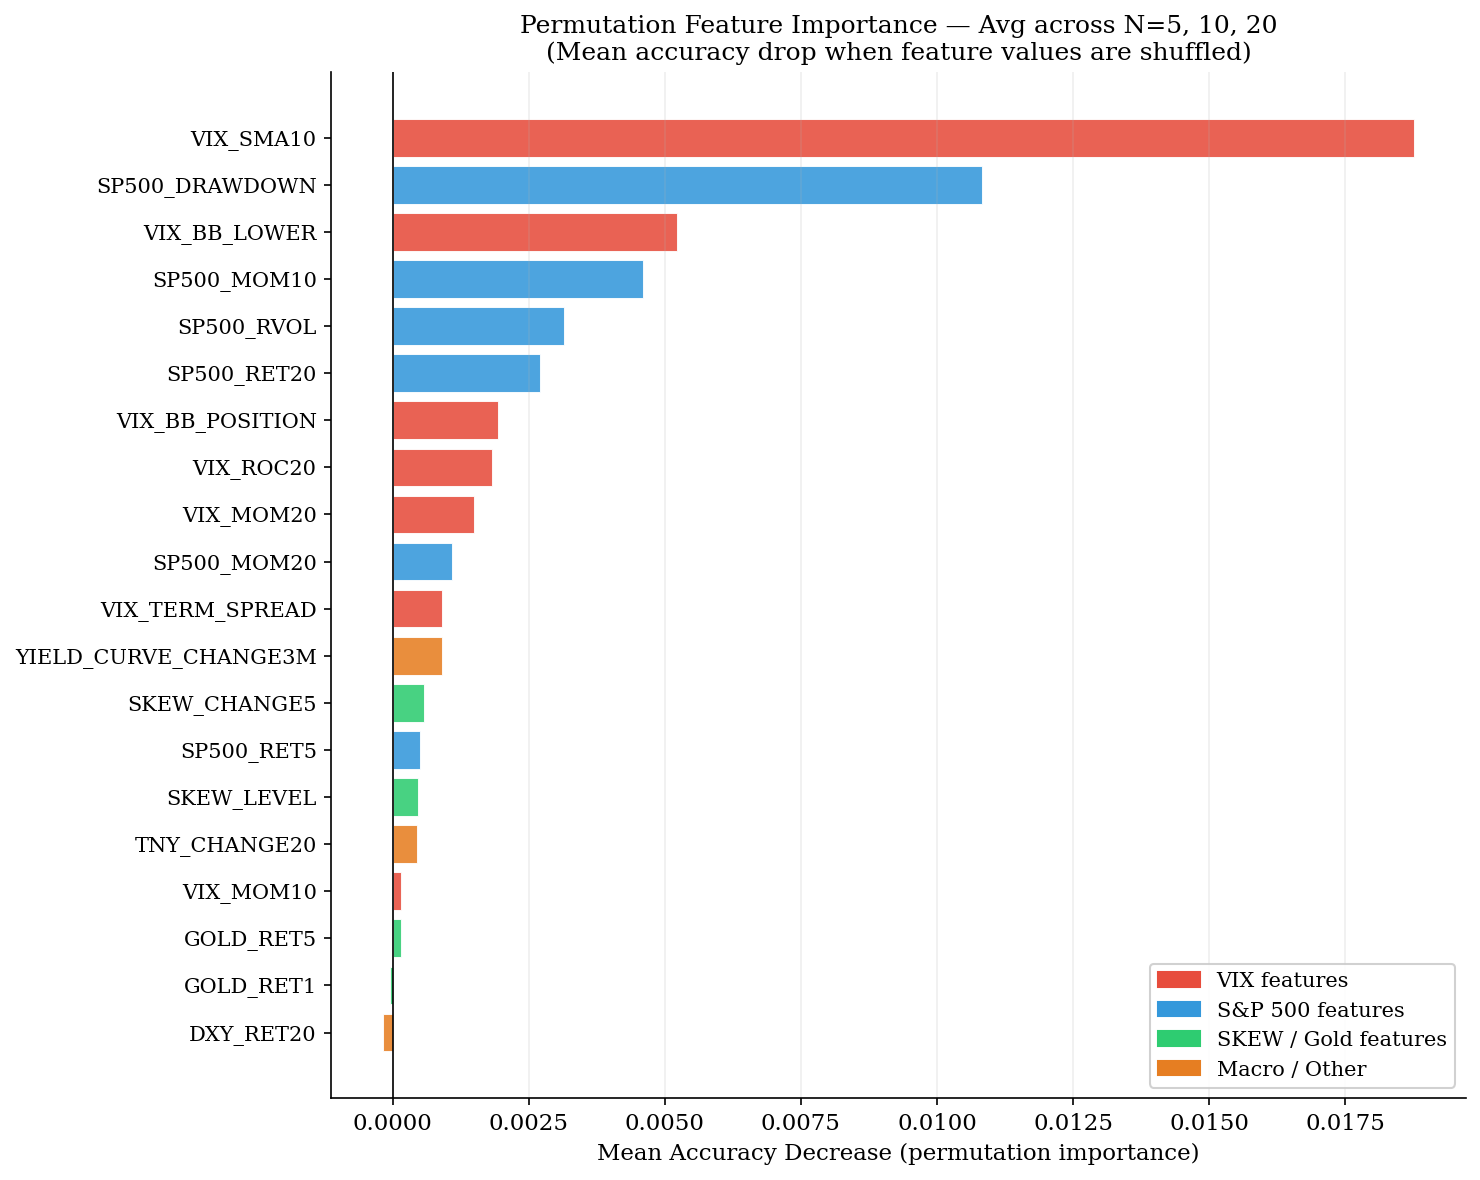
\includegraphics[width=0.75\textwidth]{permutation_importance.png}
    \caption{Permutation feature importance (mean accuracy drop when feature is shuffled), averaged across $N = 5, 10, 20$. This measure avoids the high-cardinality inflation of MDI and shifts relative emphasis toward S\&P 500 features.}
    \label{fig:fi}
\end{figure}

Permutation importance is used in preference to mean decrease in impurity (MDI) because MDI inflates the apparent importance of correlated features with high cardinality; permutation importance does not share this bias, though it too is affected by feature correlations in the sense that shuffling one member of a correlated pair leaves its partner intact. The top eight features are shown; the remaining 28 each cause less than 0.15\% average accuracy drop. VIX\_SMA10 ranks first with a 1.88\% mean accuracy drop when shuffled. S\&P 500 drawdown (SP500\_DRAWDOWN) ranks second at 1.08\%---the highest-ranked non-VIX feature---registering the largest marginal predictive contribution among non-VIX features in the fitted model. The VIX Bollinger Band cluster accounts for ranks 3 and 7.

The permutation importance values are small in absolute terms (each feature causes less than 2\% accuracy drop when shuffled), consistent with the finding that VIX autocorrelation captures most of the predictable variation. The HAR-LR baseline's competitive performance reinforces this: the marginal value of 33 additional features beyond the three-variable VIX autoregressive structure is small.

\subsection{Cost-Weighted Utility Analysis}
\label{sec:utility}

The transition analysis shows that the framework achieves 0\% accuracy on calm$\to$high spike days it covers. From a practitioner standpoint, the asymmetry between false negatives (missed spikes) and false positives (false alarms) matters: failing to predict a volatility spike is typically far more costly than issuing an unnecessary hedge. We quantify this using a cost utility function:
\begin{equation}
    U = -\frac{\text{FP} + C \cdot \text{FN}}{n_{\text{predictions}}}
    \label{eq:utility}
\end{equation}
where $C$ is the relative cost of a false negative vs.\ a false positive, and higher utility (closer to zero) is better. We compare RF selective, persistence at matched coverage, RF baseline (full coverage), and always-calm (100\% coverage, zero FP, all FN) across FN/FP cost ratios $C \in \{1, 5, 10, 20\}$ at $N = 5$ and $N = 10$.

\begin{table}[H]
\centering
\caption{Cost-weighted utility per prediction under different FN/FP cost ratios $C$. Higher utility (closer to 0) is better. Bolded entries show where persistence dominates RF selective prediction.}
\label{tab:utility}
\begin{tabular}{ccrrrr}
\toprule
$N$ & $C$ & RF Selective & Persistence & RF Baseline & Always Calm \\
\midrule
5 &  1 & $-0.081$ & $-0.087$ & $-0.166$ & $-0.301$ \\
5 &  5 & $-0.276$ & $-0.286$ & $-0.515$ & $-1.507$ \\
5 & 10 & $-0.518$ & $-0.535$ & $-0.950$ & $-3.013$ \\
5 & 20 & $-1.004$ & $-1.033$ & $-1.821$ & $-6.026$ \\
\midrule
10 &  1 & $-0.100$ & $-0.120$ & $-0.205$ & $-0.301$ \\
10 &  5 & $-0.380$ & $\mathbf{-0.326}$ & $-0.626$ & $-1.503$ \\
10 & 10 & $-0.730$ & $\mathbf{-0.584}$ & $-1.152$ & $-3.006$ \\
10 & 20 & $-1.430$ & $\mathbf{-1.100}$ & $-2.204$ & $-6.012$ \\
\bottomrule
\end{tabular}
\end{table}

\begin{figure}[H]
    \centering
    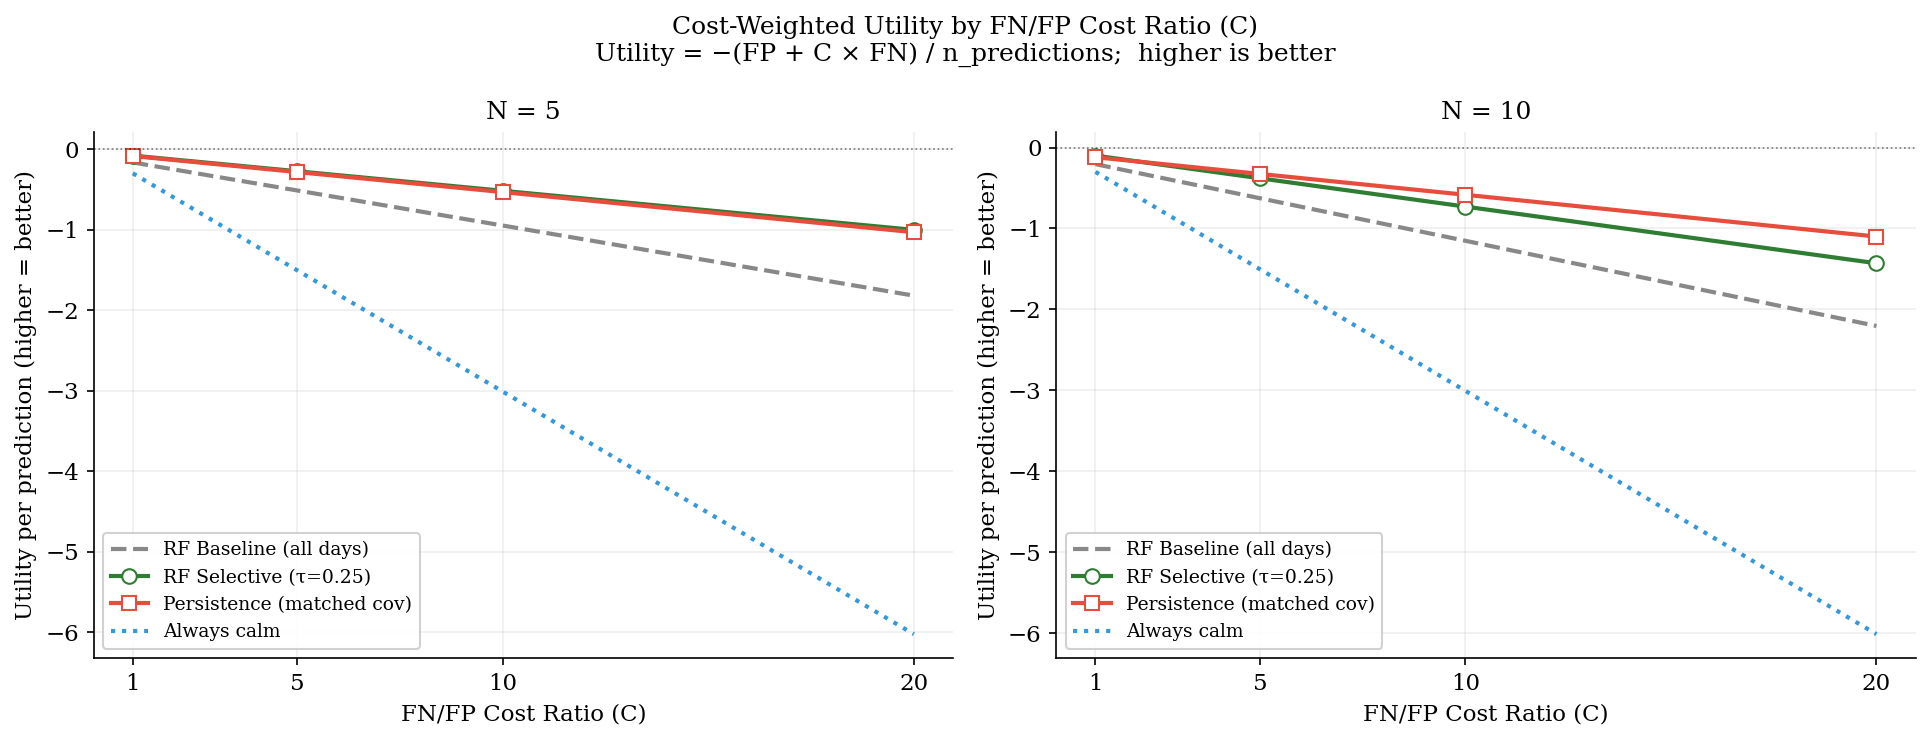
\includegraphics[width=0.85\textwidth]{cost_utility.png}
    \caption{Cost-weighted utility as a function of FN/FP cost ratio $C$ at $N = 5$ (left) and $N = 10$ (right). At $N = 10$ with $C \geq 5$, persistence at matched coverage dominates RF selective prediction.}
    \label{fig:utility}
\end{figure}

At $N = 5$, RF selective beats persistence at all cost ratios, reflecting modest precision advantages at the shortest horizon. At $N = 10$, the ordering reverses when $C \geq 5$: persistence at matched coverage achieves higher utility than RF selective prediction because the persistence baseline makes fewer false negative errors on the covered days. This result quantifies the practical implication of the 0\% calm$\to$high accuracy: the RF selective framework is utility-beneficial only when false positives are as costly as false negatives ($C = 1$). At any moderate FN/FP cost asymmetry ($C \geq 5$), a practitioner would be better served by the simpler persistence rule at $N = 10$.

%-----------------------------------------------------------------------
\section{Conclusion}
\label{sec:conclusion}
%-----------------------------------------------------------------------

This paper applies a three-part diagnostic protocol to VIX regime classification and shows that headline selective prediction accuracy reflects autocorrelation, not machine learning skill. The confidence filter achieves 0\% accuracy on every calm$\to$high transition it covers; explicit cost-weighting up to $20{\times}$ does not rescue this, confirming the failure is informational rather than objective-function-driven. A McNemar test on jointly covered days finds $b = c = 0$ at $N \geq 10$: RF and persistence make identical predictions on every shared day, so the accuracy gap is entirely composition-driven. Three-feature HAR logistic regression matches or exceeds 36-feature RF in point estimate at four of five horizons with no bootstrap-significant gap; cost-weighted utility at $N = 10$ favors persistence whenever false negatives are more costly than false alarms; and all conclusions survive excluding the 2022 bear-market period. HGB mirrors RF behavior throughout: it achieves similar selective accuracy but also suffers 50\% balanced accuracy at $N = 25$ and offers no practical advantage in walk-forward evaluation. The RF's one measurable distinction over persistence is fold-to-fold stability ($N = 5$ fold std: RF 1.7\% vs.\ persistence 3.2\%), not directional accuracy. The one exploratory exception is that model abstention carries a small independent increment beyond VIX proximity at $N = 5$ (likelihood-ratio statistic $p = 0.001$ on the evaluation sample, not a confirmatory result), but this is post-hoc and requires dedicated out-of-sample confirmation. The protocol---coverage-matched decomposition, transition accuracy audit, abstention confound test---is modular and applicable to any selective prediction system on serially correlated labels.

\subsection*{Limitations}

The feature set consists of publicly available daily market data. Calm$\to$high transitions are disproportionately triggered by exogenous shocks---geopolitical events, policy surprises, sudden liquidity crises---that leave no advance signature in daily price features. In this sense, 0\% covered accuracy on transition days is an expected structural property of the problem: the confidence filter fails not by mispredicting knowable patterns but by issuing confident wrong predictions on event-driven days it cannot distinguish from ordinary calm days. The four-year test period (June 2022--May 2026, ${\approx}1{,}000$ trading days) is underpowered for distinguishing accuracy differences of 1--3 pp under serial dependence; a longer out-of-sample window is needed to confirm directional findings.

\subsection*{Future Work}

The primary open direction is feature enrichment: incorporating event-anticipation content such as options skew dynamics, credit spreads, or order-flow imbalance that may carry advance signal about exogenous shocks. A two-stage system using the abstention rate as a leading indicator followed by a conditional spike-prediction model is a second natural direction. The diagnostic protocol developed here provides the evaluation infrastructure for either extension.

%-----------------------------------------------------------------------
\appendix
\section{Complete Feature List}
\label{app:features}

\begin{table}[H]
\centering
\caption{All 36 engineered features used as model inputs, grouped by category. All features are computed from information available at or before prediction date $t$.}
\label{tab:features}
\small
\begin{tabular}{llll}
\toprule
\# & Feature name & Definition & Category \\
\midrule
1  & VIX\_SMA10        & 10-day simple moving average of VIX                        & VIX trend \\
2  & VIX\_SMA20        & 20-day simple moving average of VIX                        & VIX trend \\
3  & VIX\_MOM10        & VIX$_t$ $-$ VIX$_{t-10}$                                  & VIX momentum \\
4  & VIX\_MOM20        & VIX$_t$ $-$ VIX$_{t-20}$                                  & VIX momentum \\
5  & VIX\_ROC10        & $({\rm VIX}_t / {\rm VIX}_{t-10}) - 1$                     & VIX momentum \\
6  & VIX\_ROC20        & $({\rm VIX}_t / {\rm VIX}_{t-20}) - 1$                     & VIX momentum \\
7  & VIX\_BB\_STD      & 20-day rolling std.\ of VIX (Bollinger bandwidth)          & VIX Bollinger \\
8  & VIX\_BB\_UPPER    & VIX\_SMA20 $+$ 2$\times$VIX\_BB\_STD                       & VIX Bollinger \\
9  & VIX\_BB\_LOWER    & VIX\_SMA20 $-$ 2$\times$VIX\_BB\_STD                       & VIX Bollinger \\
10 & VIX\_BB\_POSITION & (VIX$_t$ $-$ VIX\_BB\_LOWER) / (4$\times$VIX\_BB\_STD)    & VIX Bollinger \\
11 & VIX\_RSI14        & 14-day Relative Strength Index of VIX                      & VIX oscillator \\
12 & VIX\_MACROSS      & VIX\_SMA10 $-$ VIX\_SMA20                                  & VIX trend \\
13 & VIX\_TERM\_SPREAD & VIX3M$_t$ $-$ VIX$_t$                                      & VIX structure \\
\midrule
14 & SKEW\_LEVEL       & Raw CBOE SKEW index value                                  & Tail risk \\
15 & SKEW\_CHG5        & SKEW$_t$ $-$ SKEW$_{t-5}$                                  & Tail risk \\
16 & SKEW\_CHG20       & SKEW$_t$ $-$ SKEW$_{t-20}$                                 & Tail risk \\
\midrule
17 & SP500\_RET1       & Log return of S\&P 500 over 1 day                          & Equity \\
18 & SP500\_RET5       & Log return of S\&P 500 over 5 days                         & Equity \\
19 & SP500\_RET20      & Log return of S\&P 500 over 20 days                        & Equity \\
20 & SP500\_MOM10      & S\&P 500 price at $t$ $-$ price at $t-10$                  & Equity \\
21 & SP500\_MOM20      & S\&P 500 price at $t$ $-$ price at $t-20$                  & Equity \\
22 & SP500\_RVOL       & 20-day realized volatility of S\&P 500 daily returns        & Equity \\
23 & SP500\_DRAWDOWN   & 252-day maximum drawdown of S\&P 500                       & Equity \\
\midrule
24 & GOLD\_RET1        & Log return of gold futures over 1 day                      & Cross-asset \\
25 & GOLD\_RET5        & Log return of gold futures over 5 days                     & Cross-asset \\
26 & GOLD\_RET20       & Log return of gold futures over 20 days                    & Cross-asset \\
27 & TNY\_CHG1         & 10Y Treasury yield change over 1 day                       & Cross-asset \\
28 & TNY\_CHG5         & 10Y Treasury yield change over 5 days                      & Cross-asset \\
29 & TNY\_CHG20        & 10Y Treasury yield change over 20 days                     & Cross-asset \\
30 & DXY\_RET1         & Log return of DXY over 1 day                               & Cross-asset \\
31 & DXY\_RET5         & Log return of DXY over 5 days                              & Cross-asset \\
32 & DXY\_RET20        & Log return of DXY over 20 days                             & Cross-asset \\
\midrule
33 & FEDFUNDS\_CHG1M   & Federal Funds Rate change over $\approx$21 trading days    & Macro \\
34 & FEDFUNDS\_CHG3M   & Federal Funds Rate change over $\approx$63 trading days    & Macro \\
35 & YIELD\_CURVE\_CHG1M & T10Y2Y spread change over $\approx$21 trading days        & Macro \\
36 & YIELD\_CURVE\_CHG3M & T10Y2Y spread change over $\approx$63 trading days        & Macro \\
\bottomrule
\end{tabular}
\end{table}

%-----------------------------------------------------------------------
\bibliographystyle{plainnat}
\begin{thebibliography}{99}

\bibitem[Chen and Guestrin(2016)]{chen2016}
Chen, T. and Guestrin, C. (2016).
\newblock XGBoost: A scalable tree boosting system.
\newblock In \emph{Proceedings of the 22nd ACM SIGKDD International Conference on Knowledge Discovery and Data Mining}, pages 785--794.

\bibitem[Bartlett and Wegkamp(2008)]{bartlett2008}
Bartlett, P.~L. and Wegkamp, M.~H. (2008).
\newblock Classification with a reject option using a hinge loss.
\newblock \emph{Journal of Machine Learning Research}, 9:1823--1840.

\bibitem[Bollerslev(1986)]{bollerslev1986}
Bollerslev, T. (1986).
\newblock Generalized autoregressive conditional heteroskedasticity.
\newblock \emph{Journal of Econometrics}, 31(3):307--327.

\bibitem[Breiman(2001)]{breiman2001}
Breiman, L. (2001).
\newblock Random forests.
\newblock \emph{Machine Learning}, 45(1):5--32.

\bibitem[Chow(1970)]{chow1970}
Chow, C.~K. (1970).
\newblock On optimum recognition error and reject tradeoff.
\newblock \emph{IEEE Transactions on Information Theory}, 16(1):41--46.

\bibitem[Corsi(2009)]{corsi2009}
Corsi, F. (2009).
\newblock A simple approximate long-memory model of realized volatility.
\newblock \emph{Journal of Financial Econometrics}, 7(2):174--196.

\bibitem[Fernandes et~al.(2014)]{fernandes2014}
Fernandes, M., Medeiros, M.~C., and Scharth, M. (2014).
\newblock Modeling and predicting the CBOE market volatility index.
\newblock \emph{Journal of Banking \& Finance}, 40:1--10.

\bibitem[Geifman and El-Yaniv(2017)]{geifman2017}
Geifman, Y. and El-Yaniv, R. (2017).
\newblock Selective classification for deep neural networks.
\newblock \emph{Advances in Neural Information Processing Systems}, 30.

\bibitem[Kunsch(1989)]{kunsch1989}
Kunsch, H.~R. (1989).
\newblock The jackknife and the bootstrap for general stationary observations.
\newblock \emph{The Annals of Statistics}, 17(3):1217--1241.

\bibitem[Guidolin and Timmermann(2007)]{guidolin2007}
Guidolin, M. and Timmermann, A. (2007).
\newblock Asset allocation under multivariate regime switching.
\newblock \emph{Journal of Economic Dynamics and Control}, 31(11):3503--3544.

\bibitem[Hamilton(1989)]{hamilton1989}
Hamilton, J.~D. (1989).
\newblock A new approach to the economic analysis of nonstationary time series and the business cycle.
\newblock \emph{Econometrica}, 57(2):357--384.

\bibitem[Whaley(2009)]{whaley2009}
Whaley, R.~E. (2009).
\newblock Understanding the VIX.
\newblock \emph{Journal of Portfolio Management}, 35(3):98--105.

\end{thebibliography}

\end{document}
